% WP X: "WP name"
% Deliverable DX.Y: "Name of this deliverable"
%
% Editors: Name and Surname of the Editor
% List of Authors:
%

\documentclass{SmartReport}
\usepackage{url, rotating,todonotes}
\let\svtodo\todo\renewcommand\todo[1]{\svtodo[inline]{#1}}

\usepackage{subfig}

\begin{document}
\wpnumber{8} \wptitle{Architecture and Integration}
\instshort{ShortNameInstitution} \delnumber{8.3} \versionnumber{0.1}
\contribshort{UH}
\deltitle{Second Platform Prototype and Validation}
\delshorttitle{Platform Prototype} 
\delavail{CO}
\delstatus{F}	
\duedate{30/06/2015}
\deldate{\today}
\delowner{Iacopo Carreras, Daniele Miorandi}
\wpleader{Iacopo Carreras, UH}
\qualityassessor{Luc Moreau, SOTON}
\smartkeywords{Platform, Prototype, Integration, Validation}
\maketitle

\newcommand{\mdl}{\textsc{SmartCOM}}

\begin{smartcontributors}
%%syntax: version number & date & author (institution) & reviewer (individual)\\
%0.1 & 04/11/2014 & 
UH & Tommaso Schiavinotto, Daniele Miorandi, Iacopo Carreras\\
\end{smartcontributors}

%define the abstract
\begin{smartabstract}
This report describes the version 2.0 of the SmartSociety platform, which integrates the instantiation of the components designed and developed by the Consortium members within the framework of the technical workpackages WP2-WP7. 

The report at hand includes a revised architectural view, plus a description of the platform runtime and of the software components integrated. A brief description of the validation and testing steps carried out by developing applications on top of the platform concludes the report. 




\end{smartabstract}


\section*{List of Acronyms}
\begin{tabular}{|c|p{3cm}|p{10cm}|}
\hline 
\textbf{Acronym} & \textbf{Full Name} & \textbf{Description} \\
\hline 
\hline 
%EC & Evaluator Component & System component in charge of evaluating the outcomes of each computation task (Sec.~\ref{sec:evaluator}).\\
%\hline 
CM & Context Manager & System componet in charge of monitoring the
context the agent represented on the platform by a peer is in.\\
\hline
IM & Incentives Manager & System component in charge of managing the implementation of incentive schemes.\\  
\hline 
KB & Knowledge Base &  System component in charge of storing and managing the knowledge in the platform.\\
\hline
OM & Orchestration Manager &  System component in charge of
orchestrating the lifecycle of tasks on the SmartSociety platform. \\
\hline 
PF & Programming Framework &  System component in charge of exposing
appropriate primitives and interfaces to application developers.\\
\hline 
PM & Peer Manager &  System component in charge of managing peers.\\
\hline 
PS & Provenance Store & System component in charge of logging actions performed by platform components and peers.\\
\hline
RM & Reputation Manager & System componet in charge of handling the reputation of any system resource, including peers. \\
\hline
SmartCom & Communication Middleware & System component in charge of managing
communication channels between the platform and the peers. \\
\hline
TEM & Task Execution Manager & System component in charge of
monitoring the execution of tasks and trigger corrective actions if
needed.\\
\hline
\end{tabular}

\newpage

%%%%%%%%%%%%%%%%%%%%%%%%%%%%%%%%%%%%%%%%%%%%%%%%%%%%%%%%%%%%%%%%%%%%%%%%%%%%%%%%%%%%%%%%%%%%%%%%%%%%%%%%%%%%%%%%%%%%%%%%
%%%%%%%%%%%%%%%%%%%%%%%%%%%%%%%%%%%%%%%%

\section{Introduction}
\label{sec:intro}
This report describes the version 2.0 of the SmartSociety platform. The corresponding software components can be accessed at the following integrated repository:
\url{https://gitlab.com/smartsociety/}\footnote{A login/password has been created for reviewers: SmartSocietyReviewer/sm@rts0c13tyr3v13w3r}.%https://gitlab.com/Teudimundo/smartask}

The version 2.0 builds upon the first version, which was delivered as D8.2~\cite{D8.1}. During the period M25-M30, the integration work continued along the roadmap included in D8.2~\cite{D8.2} leading to the integration of the provenance service, to the integration of the new version of the peer manager and to a refactoring of the runtime in order to ensure alignment with the programming framework developed in WP7. Furthermore, some lab experiments were carried out to test and validate the platform functionalities and its ability to support the complete application lifecycle. 

The report is organized as follows. Sec.~\ref{sec:arch} includes the updated architectural diagrams (logical, deployment and dynamic views). Sec.~\ref{sec:sw} describes the artifacts that constitute the platform prototype. Sec.~\ref{sec:val} describes the validation and testing activities and their outcomes. Sec.~\ref{sec:concl} concludes the report providing a roadmap for activities between M30 and M48.

%Starting from the analysis of requirements and initial platform architecture in D8.1~\cite{D8.1}, WP8 undertook an intense dialogue with technical workpackages (WP2-WP7) in order to ensure full alignment of the top-level platform architecture and of the scientific and technical outcomes of WP2-WP7. The main result of this first phase was a revised architecture of the SmartSociety platform, which is presented in Sec.~\ref{sec:arch}. During the second half of the year the actual integration of components started, resulted in a 'minified' version of the platform, which integrates the Peer Manager (PM), the Orchestration Manager (OM) and the Communication Middleware (CM), plus an application runtime. For such aforementioned components, the interfaces used are summarised in Sec.~\ref{sec:apis}. The platform-level APIs and functionality are described in Sec.~\ref{sec:sw}. The missing components will be integrated during the third year according to the roadmap outlined in Sec.~\ref{sec:concl}.

% Within the SmartSociety project, Work-Package 8 (WP8) covers a twofold
% role. First, it is in charge of defining the architecture of
% the SmartSociety platform, ensuring a consistent view of the overall system, 
% as well of the components being developed by the various technical
% work-packages. Second, it aims at integrating the
% software components developed in the technical work-packages (WP2-WP7)
% into a coherent system prototype. Such prototype platform will be
% used to develop and validate the proof-of-concept applications realized in WP9.

% Within the first year of activities, only one task (T8.1, {\it Platform
% requirements analysis and design}) was active. Activities started, in
% line with the work plan, at M7. This deliverable
% includes therefore the outcomes of the activities undertaken by Consortium
% partners within the period M7-M12. 

% Activities focused on (i) the analysis of requirements for the SmartSociety platform (ii) its preliminary design in terms of system-level architecture. 

% High-level requirements were elicited by working in close cooperation with the
% other WPs. They are organized around the many heterogeneous dimensions involved in the design of a complex socio-technical system such as SmartSociety, and cover the properties
% that should be met by the final platform prototype. The analysis of the requirements represented the starting point for the design of the
% system-level architecture. \\
% The architectural design was inspired by four principles:
% \begin{itemize}
% \item {\bf Requirements:} the need to meet the requirements identified in the first part
% of the deliverable for the SmartSociety platform. Such requirements will affect the design of both the overall system, as well as of single modules and components.
% \item {\bf Integration:} the ability to provide a clear description of how the outcomes
% of the technical WPs (WP2-WP7) will be aligned and coherently integrated in the platform
% prototype.
% \item {\bf Flexibility:} supporting flexibility in the usage of the platform in order to
% enable the on-field experimental activities to be carried out for validation purposes in WP9. 
% \item {\bf 3E}: To promote the re-use of existing infrastructures, components and modules in the development process in order to meet the criteria of economy, efficiency and effectiveness. 
% \end{itemize}

% Based on these considerations, a first design of the overall platform architecture was carried out. It encompasses:
% \begin{itemize}
% \item the definition of the logical and functional role of each platform component. This includes also the preliminary identification of modules within each component, in line with the progress of single technical WPs (Logical View);
% \item the identification of how the various components interact with each other when running a computation (Dynamic View);
% \item a preliminary identification of the deployment constraints (Deployment View).
% \end{itemize}

% Finally, a sample mapping to one of the scenarios used in the first year by the Project Consortium, namely the ride sharing one, is reported. Ride sharing has been used by the Consortium as an illustrative example of a hybrid computation. This mapping is provided in order to help other WPs to achieve a better understanding of the functionalities and features to be provided by each component and of the interactions with other WPs.

% The architecture presented in this document will represent the starting point for the integration activities to be carried out in the second year of activities. The architecture will be iteratively revised, as the specifications of components by WP2-WP7 become available and scenarios and use cases get refined by WP9. The architecture of the SmartSociety platform should therefore be regarded as a reference living document, which will change and evolve over the life-time of the project. The adoption of an agile approach in the development and integration process will be adopted, with architectural design documentation getting updated at each release of the platform prototype. A first revised version of the architecture will be released together with the first prototype at M24 (D8.2). 

% The remainder of this deliverable is organized as follows. In
% Sec.~\ref{sec:requirements} we describe the requirements elicited for the
% SmartSociety platform. In Sec.~\ref{sec:design} we map such
% requirements to overall design patterns and principles, which
% constitute the basis for the architecture definition. The architecture
% is presented in terms of logical view in Sec.~\ref{sec:logical_view},
% of dynamic view in Sec.~\ref{sec:data_view} and of deployment view in
% Sec. \ref{sec:deployment_view}. A sample mapping to the ride-sharing scenario
% is provided in Sec.~\ref{sec:mapping_scenarios}.
% Sec.~\ref{sec:conclusions} concludes the deliverable defining a
% roadmap for the activities of WP8 in the second year of the project. 


%%%%%%%%%%%%%%%%%%%%%%%%%%%%%%%%%%%%%%%%
%%%%%%%%%%%%%%%%%%%%%%%%%%%%%%%%%%%%%%%%%%%%%%%%%%%%%%%%%%%%%%%%%%%%%%%%%%%%%%%%%%%%%%%%%%%%%%%%%%%%%%%%%%%%%%%%%%%%%%%%
\newpage


%%%%%%%%%%%%%%%%%%%%%%%%%%%%%%%%%%%%%%%%%%%%%%%%%%%%%%%%%%%%%%
\section{Platform Architecture}
\label{sec:arch}
This section describes the SmartSociety platform architecture at M30. In line with the iterative approach pursued by the Consortium, the description is a snapshot of the current status of project activities in terms of integration of technology and software modules developed, and will evolve during the remainder of project lifetime according to the roadmap described in Sec.~\ref{sec:concl}.

A simplified, high-level view of the SmartSociety platform architecture is presented in Fig.~\ref{fig:architecture}~\cite{scekic_soca2015}. 
%The architecture is designed to be fully distributed and scalable. 
The rectangle boxes represent the key platform components. All components expose RESTful APIs. The deployment can be distributed. 
%They can be deployed distributively, as all components expose (private or public) RESTful APIs. %The principal component-interoperability channels are denoted with double-headed arrows in the figure. 
%Communication with peers is additionally supported via popular commercial protocols to allow a broader integration with existing communication software and 
In order to ease inclusion of peers into the platform, interaction via popular commercial protocols and communication software is also supported.

\begin{figure}[t]
 \centering
 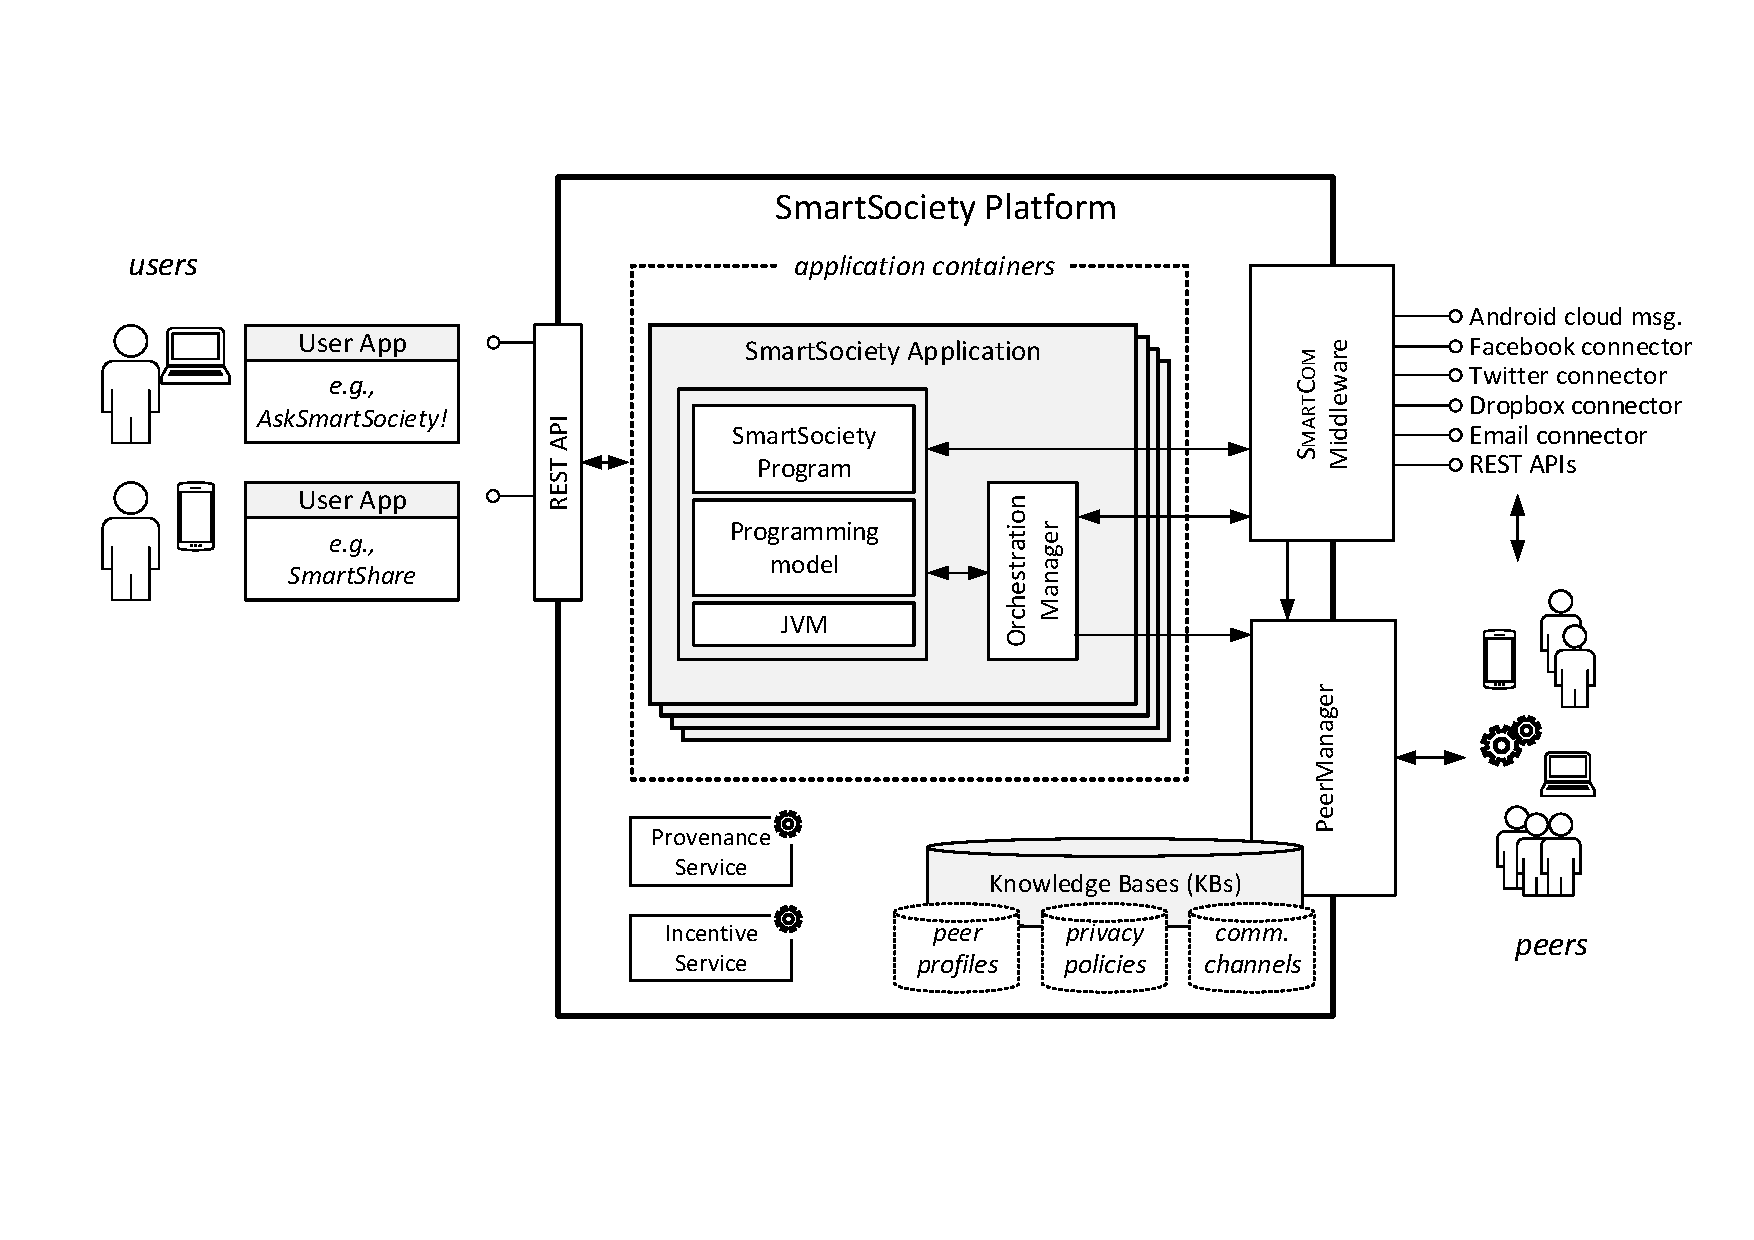
\includegraphics[width=0.8\linewidth]{figs/platform-architecture}
 \caption{SmartSociety platform users and architecture.}
 \label{fig:architecture}
\end{figure}

User applications contact the platform through the REST API component.
All incoming user requests are served by this module that %verifies their correctness and 
dispatches them to the appropriate platform application, which will be processing and responding to them. 
The platform applications run sandboxed in Docker \footnote{\url{https://www.docker.com/}} containers. The applications can be deployed on different (virtual) machines.
%
%
%The first time a platform application is run the container will take care of informing the \emph{PeerManager (PM)} component to set up (register) appropriate application, peer and collective profiles required by the application. 
Applications request from the Peer Manager a set of permissions for accessing and manipulating personal private data of peers. The Peer Manager can shortly be described as the central information system of the platform, managing all peer and application information, and allowing privacy-aware access and sharing of the data among platform components. 
%
The platform application %is a Java application 
makes use of SmartSociety platform's programming libraries, allowing the developer to execute collective-based tasks on the platform. %The developer is offered a complete \emph{programming model}\footnote{Description of the programming model is currently in submission preparation and can be made available to the reviewers upon request.} and appropriate high-level language constructs.
% for creating and executing collaborative human-machine applications. 
%
Each platform application features a dedicated \emph{Orchestration Manager (OM)} component. The OM is the component in charge of preparing and orchestrating collaborative activities among peers. Performing these functionalities requires the OM to heavily use the Peer Manager and \mdl{} Middleware components. 

% During the second year of project activities integration activities
% started. In the integration process, the architecture initially
% presented in Deliverable D8.1 was deeply revised. This process was
% required in order to align the activities carried out within the
% project's technical work packages (WP2-WP7) and to ensure
% interoperability among the components developed by the various
% partners. In this section we briefly present the architecture as it
% currently stands (at M24). No major changes are currently foreseen,
% even if ---given the research-oriented nature of the SmartSociety
% project--- this cannot be guaranteed. In this sense, the architectural
% specifications of the SmartSociety platform have to be seen as a live document, which reflects the
% actual progress of the research activities carried out by Consortium
% partners. 

%\subsection{Logical View}
%The logical view of the SmartSociety platform is presented in Fig.~\ref{fig:logical_view}. %The Consortium has identified 9 key
%components which jointly provide the required system-level functionality.

%\begin{sidewaysfigure}
%\begin{figure}[!hbt]
% \centering
% 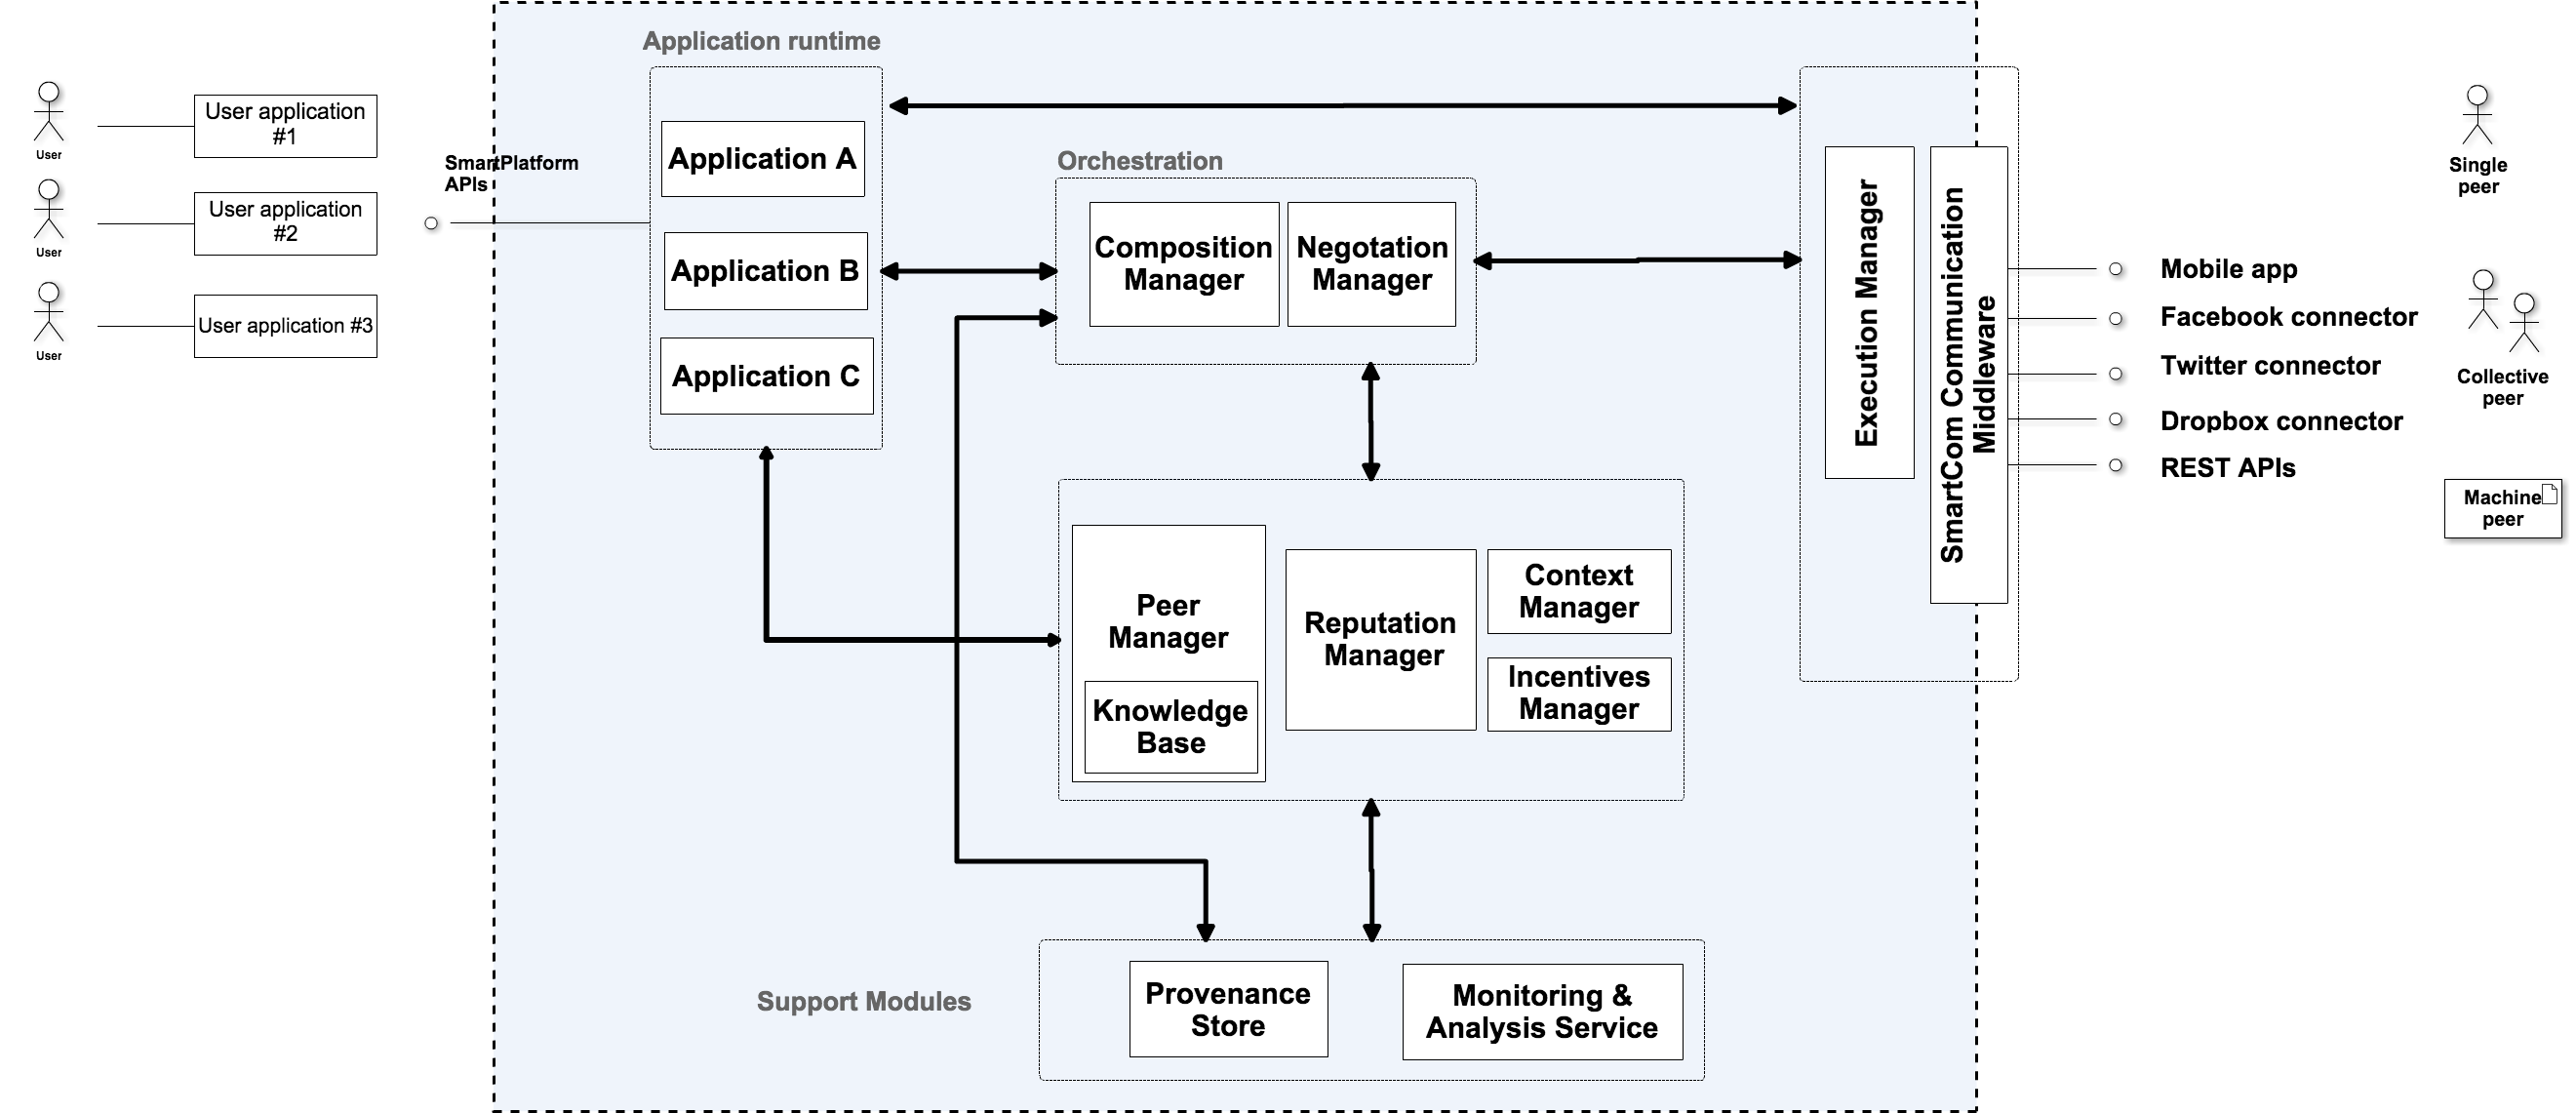
\includegraphics[width=1\textwidth]{figs/functional_diagram}%logical_view.pdf}
% \caption{SmartSociety logical view.}
% \label{fig:logical_view}
%\end{figure}
%\end{sidewaysfigure}

%\todo{Update ref to figure (take from collaboratecom paper) + shorten description of components}
A brief description of the functionality of the components integrated is reported here for the sake of completeness.
%The core components which are part of the revised version of the SmartSociety are the following:
\begin{itemize}
\item \textbf{Application Runtime}: this is the component providing the support logic enabling peers to execute tasks. The runtime provides handlers for interacting with the various internal components provided by the SmartSociety platform. In the current version (see~\ref{sec:sw} for more details on this and on the impact of the programming framework) the Application Runtime provides the main endpoint for external applications to interact with the SmartSociety platform. %The Application Runtime is developed within WP8. 

\item \textbf{Orchestration Manager}: it provides two key functionalities: composition and negotiation~\cite{D6.2}. Composition takes task requests as inputs and generates tasks by solving constraint satisfaction problems specific to each application, potentially interacting with the peer manager (so that peer with certain capabilities can be identified) and the reputation service (so that the reputation of the capable peers can be obtained). The composition determines (i) the peers which can potentially execute such task, and (ii) the necessary interactions and/or external services which are needed to execute such task.  The negotiation manager is in charge of handling the negotiation process with peers in order to ensure that the services and resources required to carry out the task are actually present. %The Orchestration Manager (OM) is developed within WP6 and its description can be found in~\cite{D6.2}.

\item \textbf{Peer Manager}: it is responsible for managing peer-related information~\cite{D4.3}. This includes their profile, as well as any other information which will be used by the Orchestration Manager for identifying possible peers that can execute a given task.  It maintains a profile of each peer, which
represents a model thereof in terms of knowledge, resources and
capacity. It provides a peer search functionality that is used by the Orchestration Manager to create compositions. Besides individual peers, the Peer Manager also manages collectives, which are groups of peers characterized by specific properties. %Besides managing peer-related information, 
The Peer Manager includes a set of mechanisms for ensuring the user's privacy~\cite{D4.3}.
%s also in charge of protecting the user's privacy. 
%The Peer Manager embeds a Knowledge Base (KB), which contains an agreed ontology about peers, task, workflows, incentives, etc. The KB provides the domain terminology, as well as all the semantic relations between terms. The KB is responsible for ensuring that all component share a common understanding of the inputs/outputs between any two parties of the platform. The overall KM is divided into domains, which allow to capture the diversity of the entities being part of SmartSociety. A semantic reasoner will allow to perform semantic queries over the KB. %The Peer Manager (PM) is developed within WP4 and its description can be found in~\cite{D4.3} .

\item \textbf{Task Execution Manager:} %\todo{Add description, take from slides resulting from the Frankfurt meeting with WP3/WP6} 
The TEM takes as input a description of the task under execution and data about the actual status of peers (mediated by the PM) to understand the level of completion and to trigger, if needed, appropriate actions by the OM.

\item \textbf{Context Manager}: it is responsible for monitoring the context the agent represented on the platform by a peer is in~\cite{D3.2}. For an individual human agent, this includes, e.g., tracking the location and recognizing the activity the agent is currently involved in. This can be further used to trigger context adaptation in applications. %The Context Manager (CM) is developed within WP3 and a high-level description can be found in~\cite{D3.2}.

\item \textbf{Reputation Manager}: it handles the reputation of any system resource, including peers ~\cite{D2.3}. It computes the reputation of a given peer based on feedback from other peers. % and users. %It uses data from the provenance store in order to carry out the computation. Reputation is based on various metrics that the system will be able to compute, starting from peers' execution of tasks. 
Reputation information can be exposed directly to application users or used by the PM in the selection of suitable peers for a given task. %The Reputation Manager (RM) is developed within WP2. A description of the RM can be found in ~\cite{D2.3}.

%\item \textbf{Knowledge Base}: it is shared among the various components of the platform, and contains an agreed ontology about peers, task, workflows, incentives, etc. It provides the domain terminology, as well as all the semantic relations between terms. In particular, the knowledge base is responsible for ensuring that all component share a common understanding of the inputs/outputs between any two parties of the platform. The overall knowledge base will be divided into domains, which allow to capture the diversity of the entities being part of SmartSociety. A semantic reasoner will allow to perform semantic queries over the knowledge base.

\item \textbf{Provenance Service}: it logs descriptionf of actions performed by platform
components and peers, as well as information flows between them, according to the W3C PROV recommendation~\cite{D2.2}. In particular, the provenance store is the component responsible for keeping a record of how the overall compositions are being created, executed and how the data managed by the platform is being transformed. %It will play a fundamental role in the evaluation of peers reputation. %, as well as in ensuring that the system as a whole enforces the proper privacy constraints imposed by the peers.
%It further supports an explanation service, which is able to visualize provenance trails and convert them in natural language. The Provenance Store (PS) is developed within WP2. A description of the PS can be found in~\cite{D2.2}.

\item {\bf Monitoring and analysis service}: it logs and monitors the platform jobs and can be used by platform administrators to perform root-cause analysis and to extract analytics on the performance of the system. 

\item {\bf Incentives manager}: it manages incentives and
interventions that can be used to achieve higher quality results. Incentives %can play a twofold role in SmartSociety. First, they 
can be used to stimulate the participation of a peer (or a collective) in the execution of a given task 
%. Second, they 
or can be used to define specific strategies for community engagement. %This will play a fundamental role in maintaining the peers community active over time. The Incentives Manager (IM) is developed within WP5.
\end{itemize} 	


% \subsection{Deployment View and Network Diagrams}
% The SmartSociety platform has been designed according to REST architectural principles, with the aim of supporting flexibility in the deployment model. %This means that 
% The platform seamlessly supports both single-tenant as
% well as multi-tenant deployment models. %Also, 
% The platform components
% can be centralised on a single infrastructure or can be distributed
% across different servers. \todo{update diagram}
% %The choice of the specific deployment model
% %to be used depends on technical as well as business considerations. In
% %the remainder of this section we present, as a use case, the current
% %deployment utilised for integration, testing, validation and
% %experimentation purposes. This is by no means to be considered the
% %only model supported, but it provides an illustrative example of a
% %supported configuration. 

% \begin{figure}[!hbt]
%  \centering
%  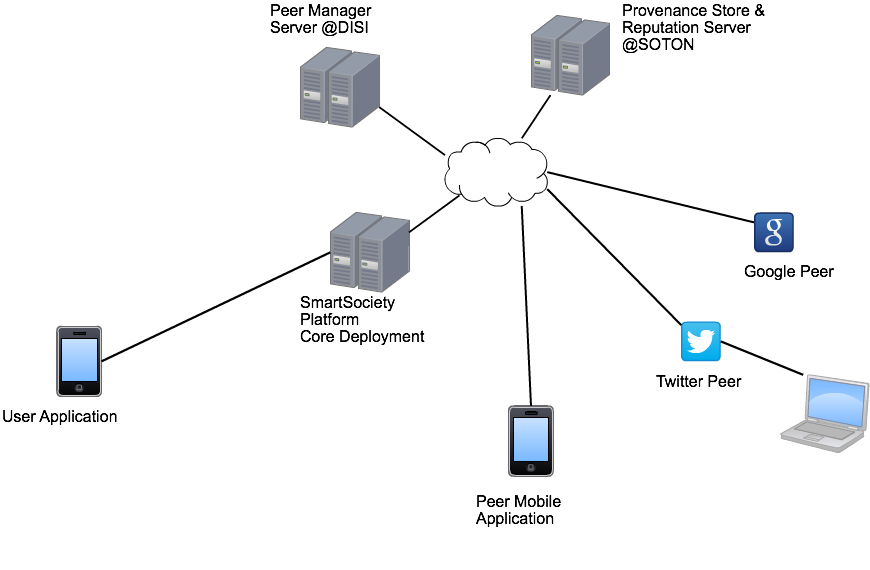
\includegraphics[width=1\textwidth]{figs/netDiagram}
%  \caption{SmartSociety platform: network diagram}
%  \label{fig:netDiagram}
% \end{figure}

% A sample network diagram is reported in Fig.~\ref{fig:netDiagram}. The end user in this case interacts with a User Application running on her smartphone. The mobile app interacts with the Application residing in the SmartSociety Platform Core Deployment. %Some of the components reside on different servers; 
% In this sample case the PM is hosted by partner DISI and the PS and RM are hosted by partner SOTON. The Core Deployment further manages interactions with peers (through the CM). In this case we have a human agent which interacts through a Peer Mobile Application, a machine peer (Google) and a machine peer (Twitter) which then reaches out to human agents interacting with it through any Twitter client.



% The corresponding deployment diagram is reported in Fig.~\ref{fig:deployDiagram}. Here it can be seen that the core deployment server hosts four key components, i.e., the incentives manager, the communication middleware, the orchestration manager and the application container (where the application is executed). On the end user smartphone, besides the user application (client), the client of the context manager is also  deployed. The CM client interacts with the corresponding server-side component deployed on the DISI server, where the PM is also hosted. The PS and RM are on the SOTON server. A third-party server is used to host both Google and Twitter peer, which then connect to the corresponding web service. \todo{update diagram}
% \begin{sidewaysfigure}
% %\begin{figure}[!hbt]
%  \centering
%  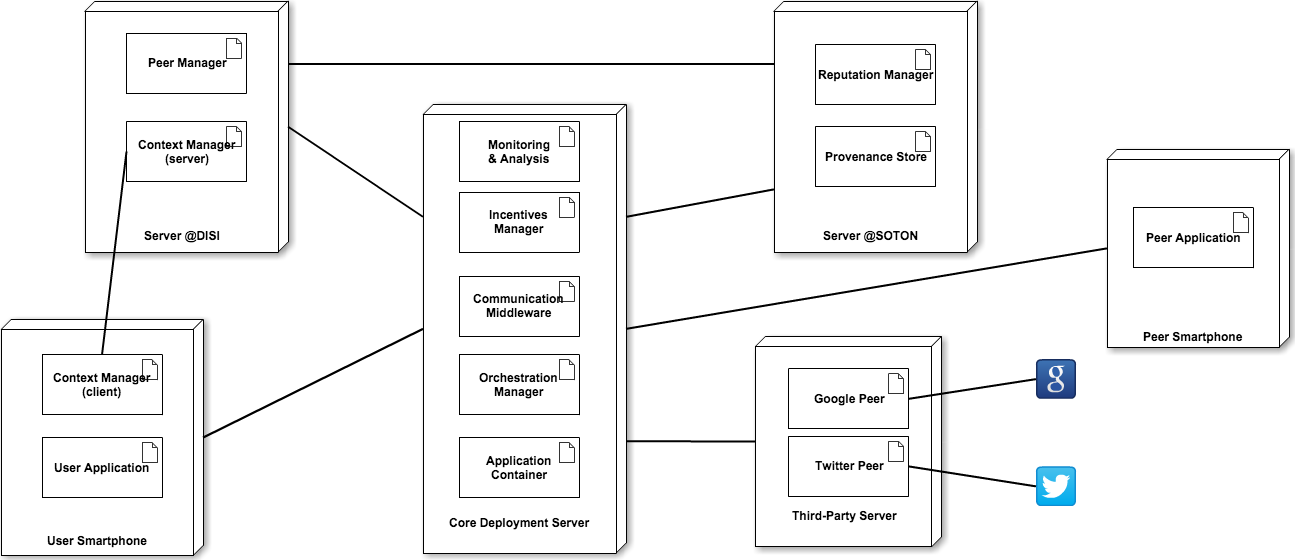
\includegraphics[width=1\textwidth]{figs/deploymentView}
%  \caption{SmartSociety platform: deployment diagram}
%  \label{fig:deployDiagram}
% %\end{figure}
% \end{sidewaysfigure}

% \subsection{Dynamic View}
% Fig.~\ref{fig:dynamic_view} provides a sample dynamic view of how the various components of the SmartSociety platform interact with each other, when running an application based on SmartSociety.\footnote{For the sake of clarity, and as these were developed while integrating the first version of the platform, only interactions among the user application, application, orchestration manager, peer manager, communication middleware and human agents are reported.} \todo{update diagram}
% \begin{sidewaysfigure}
% %\begin{figure}[!hbt]
%  \centering
%  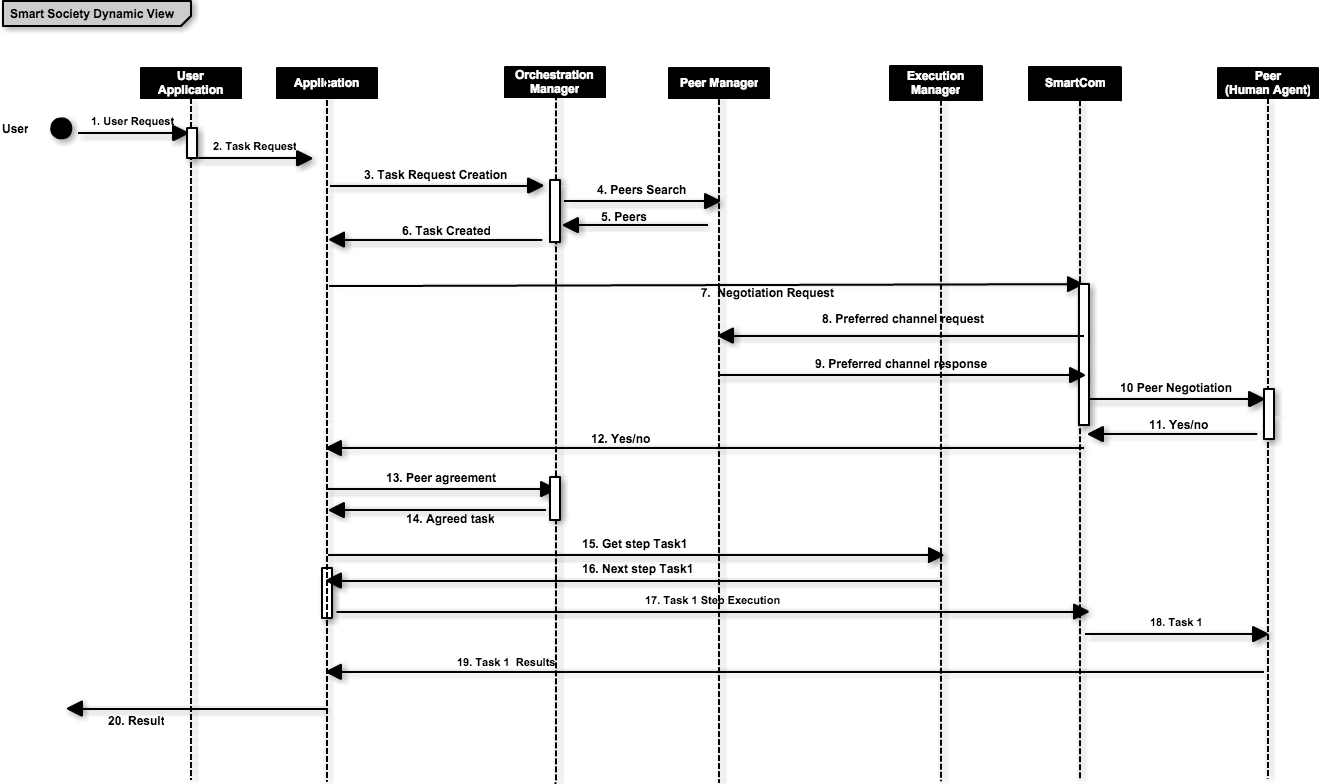
\includegraphics[width=1\textwidth]{figs/dynamic_view}
%  \caption{SmartSociety dynamic view .}
%  \label{fig:dynamic_view}
% %\end{figure}
% \end{sidewaysfigure}

% The sequence diagram can be summarized by the following steps:
% \begin{itemize}
% \item Platform invocation (step 1): the starting point is a user application (e.g., a mobile application) which is exploiting the SmartSociety platform for running a human computation task (refer to Sec.~\ref{sec:asksmartsoc} for a more concrete example). The request is directed towards an application deployed in the SmartSociety application container and providing the necessary support for executing the requested task. The invocation will contain all the necessary metadata, including a complete description of the task, according to the APIs offered by the application running in the platform.

% \item Composition request (steps 2-6): the application, after receiving the request from the user application, converts it into a \textit{composition job request}. A composition is the request to create a composition of peers/collectives capable of executing the task. The composition job request happens through %the programming abstractions provided by 
% the runtime, which allows to fully characterize the task that needs to be executed. Creating a composition involves querying the Peer Manager for identifying peers capable (individually or all together) to perform the given task\footnote{Note that also the Reputation Manager can be queried during this process. This is not reported in the diagram for the sake of simplicity, and as it reflects the current integrated components.}. Once the composition is identified, it is returned to the application, together with a pointer to the peers involved in it.

% \item  Negotiation (steps 7-14): the application then negotiates with peers the participation of the agents they represent in a given task. This is mediated/facilitated by the Orchestration Manager. Such negotiation occurs for every single peer involved in the identified composition. The negotiation with peers also involves the identification of the channel preferred by the peer to receive a given task (e.g., email, social, mobile app in the case of human agent). In this phase, the SmartCom communication middleware is exploited to facilitate the interaction with peers. At the completion of this phase, the Orchestration Manager is notified about the successful completion of the negotiation.

% \item Execution (steps 15-20): once the composition has been successfully identified and agreed with peers, the execution of the task can starts. This can be based over multiple steps and is managed by the Application, exploiting the programming framework provided be the application runtime. This phase concludes with the complete execution of the submitted task. Results are then returned to the User application that has initiated the request.

% \end{itemize}


% % The SmartSociety platform is meant to support a rather wide range of
% % social computation patterns (or templates). In order to provide
% % insight into the flexibility of the platform and the actual
% % interworking of components, we have developed sequence diagrams for two
% % 'extreme' applications:
% % \begin{itemize}
% % \item SmartShare is a ridesharing system able to account for user's
% % preferences and to compute recommendations based on the feedback
% % provided by other service users. It is what we call a 'full
% % negotiation' scenario, in which the computational task of finding an
% % agreement on the rides is left to individuals and collectives. The
% % platform in this case is used to carry out administration tasks, in
% % particular keeping track of the rides and ride requests, their status
% % and to maintain reputation of drivers and passengers.
% % \item AskSmartSociety! is a Q\&A service supporting hybridity. The
% % computational pattern here is that typical of micro-tasking
% % applications (\'a la Mechanical Turk, roughly speaking), where the
% % task in this corresponds to a question to be answered. The service
% % supports hybrid computation in that questions can be transparently
% % provided by machine peers or human peers. Quality criteria can be
% % specified in order to define when a chosen answer has to be presented
% % to the user. 
% % \end{itemize}
% % In the following we present details about the two aforementioned
% % applications. 
% % \subsubsection{Example: SmartShare}
% % \begin{figure}
% % \centering
% % 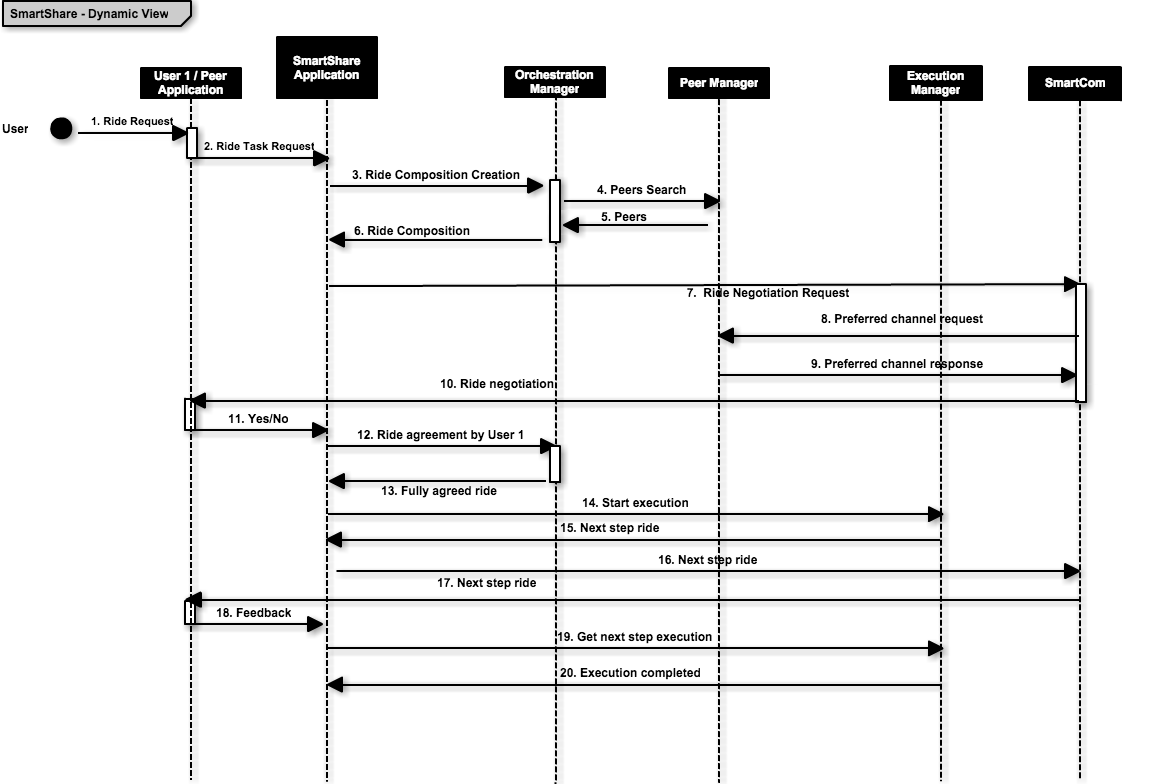
\includegraphics[width=0.9\textwidth]{./figs/sequenceRide}
% % \caption{Sequence diagram of the SmartShare application.}
% % \label{fig:dynamic_share}
% % \end{figure}

% % \subsection{Example: Ask SmartSociety}\label{sec:asksmartsoc}
% % \textit{Ask SmartSociety} is a simple Questions and Answer service enabled by the SmartSociety platform which has been used as the benchamark for implementing the initial version of the SmartSociety platform. It focus on tourism, which is the reference domain to be used for validating the SmartSociety vision.\\
% % Ask SmartSociety! will be a service where users can post questions in natural languages and peers can provide answers. Peers providing answers can be humans (individuals or collectives) as well as machines (intelligent software agents). Peers can compose (forming collectives, hybrid or not) to provide answers. Answers can be ranked based on the reputation of the peers or on community ranking (similarly to stackoverflow). In some instances the user issuing the question can select an answer and provide feedback on the peer providing it.
% % Two examples (grounded in the tourism application scenarios) can help in understanding the features of the Ask SmartSociety! service:

% % \textit{Next week Peter will fly to Venice. He will be busy in meetings during the day but wants to explore some ‘hidden’ places at night. He could well explore various online tourist sites but he prefers to ask experts and local people. He could also google for relevant content, but he does not actually need an answer right away, he just needs to get it in one week. And having one system which allows him to query local experts, web-based recommendation services and incoming tourism institutions looks definitely appealing to him!
% % Alice is visiting Milano during the next week. It is his first time in Milan, and she is looking for a restaurant in the city centre. Since it is spring time, she would love eat outside and therefore  find a restaurant with a garden. Alice is also celiac, and she needs to find restaurants, which do have gluten free menus. She relies on the Ask SmartSociety! application for retrieving some suggestions on where to have dinner during her stay in Milan. She is looking for unconventional recommendations.}


% % \begin{figure}
% % \centering
% % 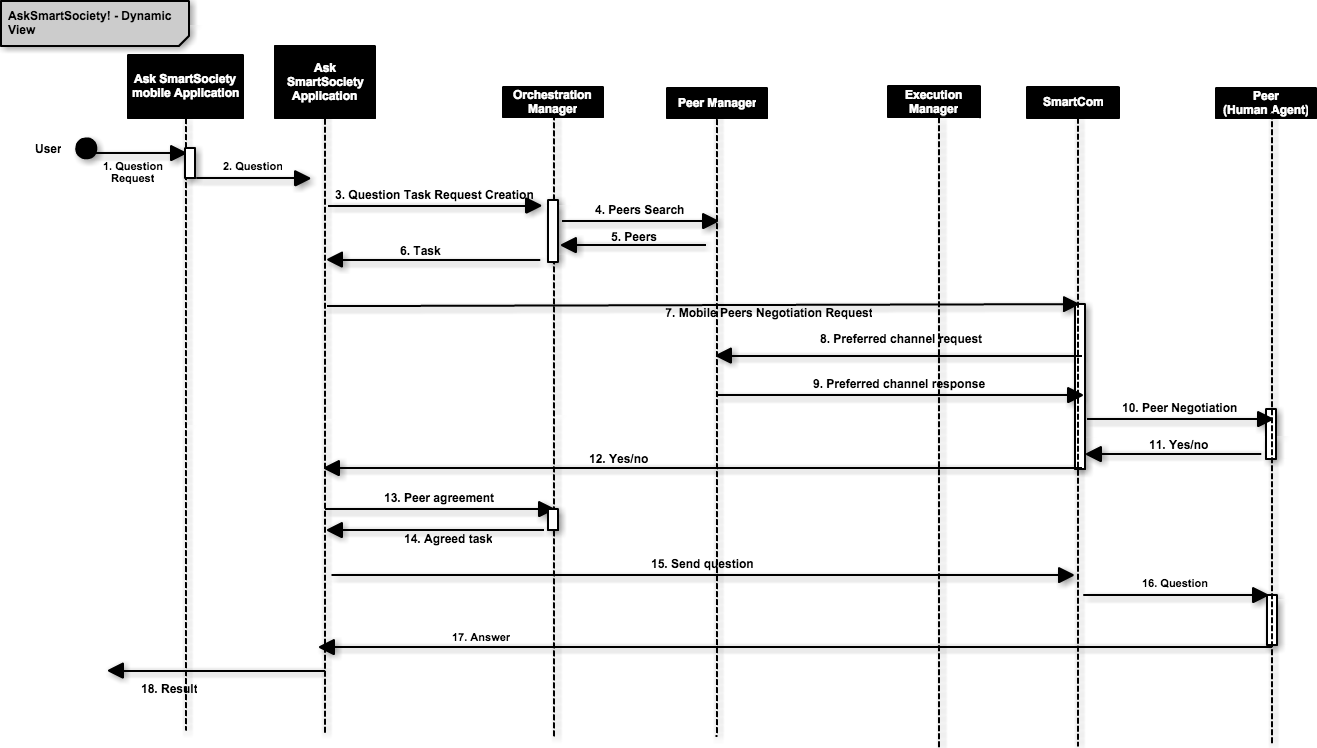
\includegraphics[width=0.9\textwidth]{./figs/sequenceAsk}
% % \caption{Sequence diagram for AskSmartSociety! applications.}
% % \label{fig:dynamic_ask}
% % \end{figure}
%%%%%%%%%%%%%%%%%%%%%%%%%%%%%%%%%%%%%%%%%%%%%%%%%%%%%%%%%%%%%%
\newpage

% %%%%%%%%%%%%%%%%%%%%%%%%%%%%%%%%%%%%%%%%%%%%%%%%%%%%%%%%%%%%%%
% \section{Mapping to the Application Scenarios}
% \label{sec:mapping}
% The SmartSociety platform is meant to support a rather wide range of
social computation patterns (or templates). In order to provide
insight into the flexibility of the platform and the actual
interworking of components, we have developed sequence diagrams for two
'extreme' applications:
\begin{itemize}
\item AskSmartSociety! is a Q\&A service supporting hybridity. The
computational pattern here is that typical of micro-tasking
applications (\'a la Mechanical Turk, roughly speaking), where the
task in this corresponds to a question to be answered. The service
supports hybrid computation in that questions can be transparently
provided by machine peers or human peers. Quality criteria can be
specified in order to define when a chosen answer has to be presented
to the user. The scenario was used as the reference benchmark for the integration work carried out in WP8.

\item SmartShare is a ridesharing system able to account for user's
preferences and to compute recommendations based on the feedback
provided by other service users. It is what we call a 'full
negotiation' scenario, in which the computational task of finding an
agreement on the rides is left to individuals and collectives. The
platform in this case is used to carry out mainly administration tasks, in
particular keeping track of the rides and ride requests, their status
and to maintain reputation of drivers and passengers. In this setting, in particular, the OM is responsible for different kinds of synchronisation during composition, negotiation, deletions, etc. This synchronisation process plays a key role in this scenario in that it enables notifying the end users that a change has taken place. 
\end{itemize}
In the following we present details about the two aforementioned
applications. 


\subsection{Example: Ask SmartSociety}\label{sec:asksmartsoc}
\textit{Ask SmartSociety} is a simple Questions and Answer service enabled by the SmartSociety platform which has been used as the benchmark for implementing the initial version of the SmartSociety platform. It focus on tourism, which is the reference domain to be used for validating the SmartSociety vision.\\
Ask SmartSociety! will be a service where users can post questions in natural languages and peers can provide answers. Peers providing answers can represent humans (individuals or collectives) as well as machines (intelligent software agents). Peers can compose (forming collectives, hybrid or not) to provide answers. Answers can be ranked based on the reputation of the peers or on community ranking (similarly to stackoverflow). In some instances the user issuing the question can select an answer and provide feedback on the peer providing it.
Two examples (grounded in the tourism application scenarios) can help in understanding the features of the Ask SmartSociety! service:

\textit{Next week Peter will fly to Venice. He will be busy in meetings during the day but wants to explore some ‘hidden’ places at night. He could well explore various online tourist sites but he prefers to ask experts and local people. He could also google for relevant content, but he does not actually need an answer right away, he just needs to get it in one week. And having one system which allows him to query local experts, web-based recommendation services and incoming tourism institutions looks definitely appealing to him!
Alice is visiting Milano during the next week. It is his first time in Milan, and she is looking for a restaurant in the city centre. Since it is spring time, she would love eat outside and therefore  find a restaurant with a garden. Alice is also celiac, and she needs to find restaurants, which do have gluten free menus. She relies on the Ask SmartSociety! application for retrieving some suggestions on where to have dinner during her stay in Milan. She is looking for unconventional recommendations.}

Fig.~\ref{fig:dynamic_ask} illustrates how SmartSociety dynamic view is instantiated in the case of the \textit{AskSmartSociety!} application.

\begin{sidewaysfigure}
%\begin{figure}[!hbt]
\centering
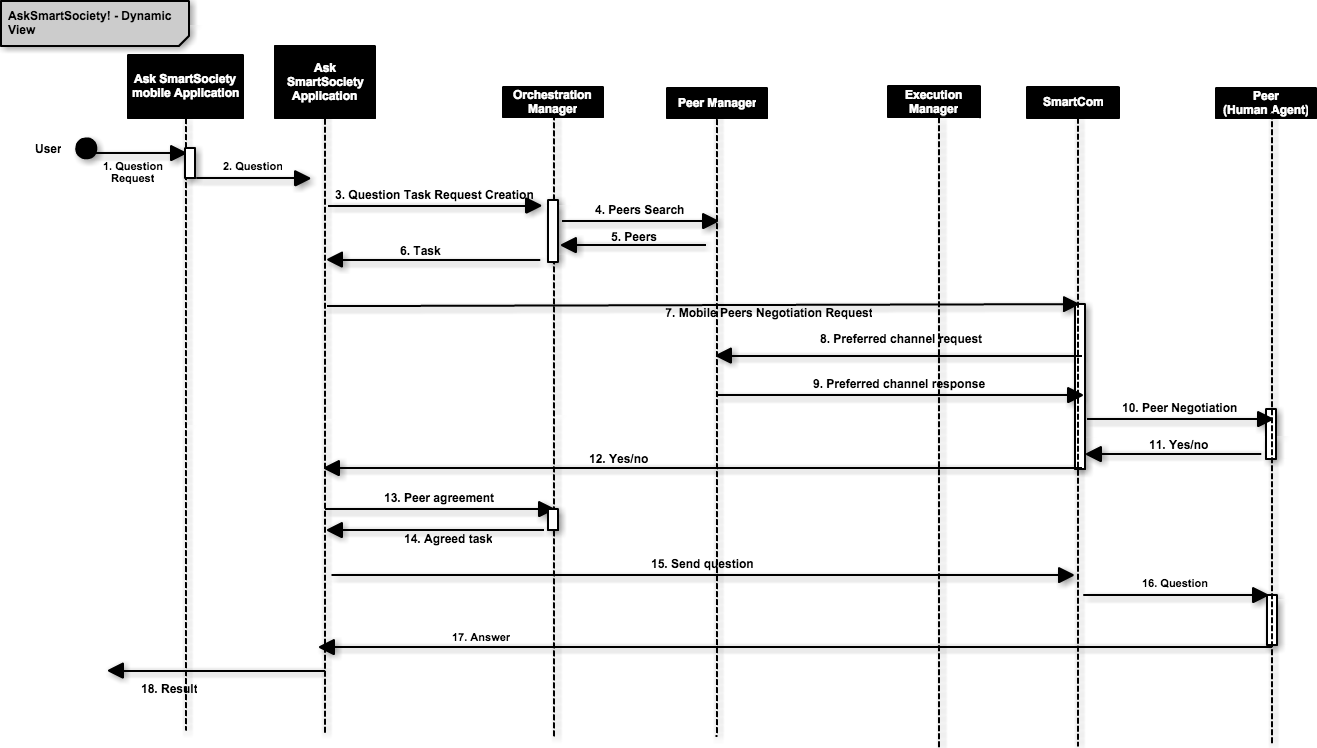
\includegraphics[width=0.9\textwidth]{./figs/sequenceAsk}%ask/ask_dynamic}
\caption{Sequence diagram for \textit{AskSmartSociety!}}
\label{fig:dynamic_ask}
\end{sidewaysfigure}

Compared to the overall sequence diagram of Fig.~\ref{fig:dynamic_view}, this is a rather simplified use case where the user application consists of a mobile application through which users can post question. The question is dispatched to the corresponding application hosted in the runtime. Such application transforms the question into a computational task to be executed by peers. Such computational task is handled by the Orchestration Manager, which identifies the most suitable composition for completing the task by querying the Peer Manager. As an example, if the question regards restaurants, the Orchestration Manager might decide to use machine peers such as, e.g., TripAdvisor or Yelp, in combination with some \textit{local knowledge} provided by human peers living in the region where the request was created. Once the composition has been created, the application recruits the peers for the execution of the task. This could potentially involve the use of incentives in order to motivate peers participation.\\
After peers have been signed up for the given task, the task execution starts. In this case, the question is sent to the peer over the preferred communication channel. In the case of machine peer, this corresponds to the proper API endpoint, whereas in the case of human peers it could be a mobile application. In the implemented scenario, we used a Twitter peer which used a hashtag to collect recommendations and a mobile application, through which users could receive questions and provide answers. In the current implementation, the Execution Manager functionality is embedded in the application itself, which interacts directly with peers exploiting the SmartCom functionalities.\\
Once the task is completed, and the answers are collected, the outcome of the computation is delivered to the users originally posting the question.

AskSmartSociety! has been prototyped to be used as both a driver of the integration process as well as to demonstrate the ability of the platform to support hybridity. Indeed, in the current prototype questions can be seamlessly answered by machine peers (in particular using the Google Search functionality) as well as human peers (using a purposeful developed mobile application). Further, a Twitter peer was developed; this is formally a machine peer, which is used to further distribute the task (in the form of the original question) to human peers, aggregating answers and feeding them back to the application. In Fig.~\ref{fig:askpeer} we display the user interface implemented in the mobile app used for testing and demonstration purposes. 
% the UX design that has been conducted for the mobile application.


\begin{figure}[!bht]
    \subfloat[Question form\label{subfig-1:dummy}]{%
      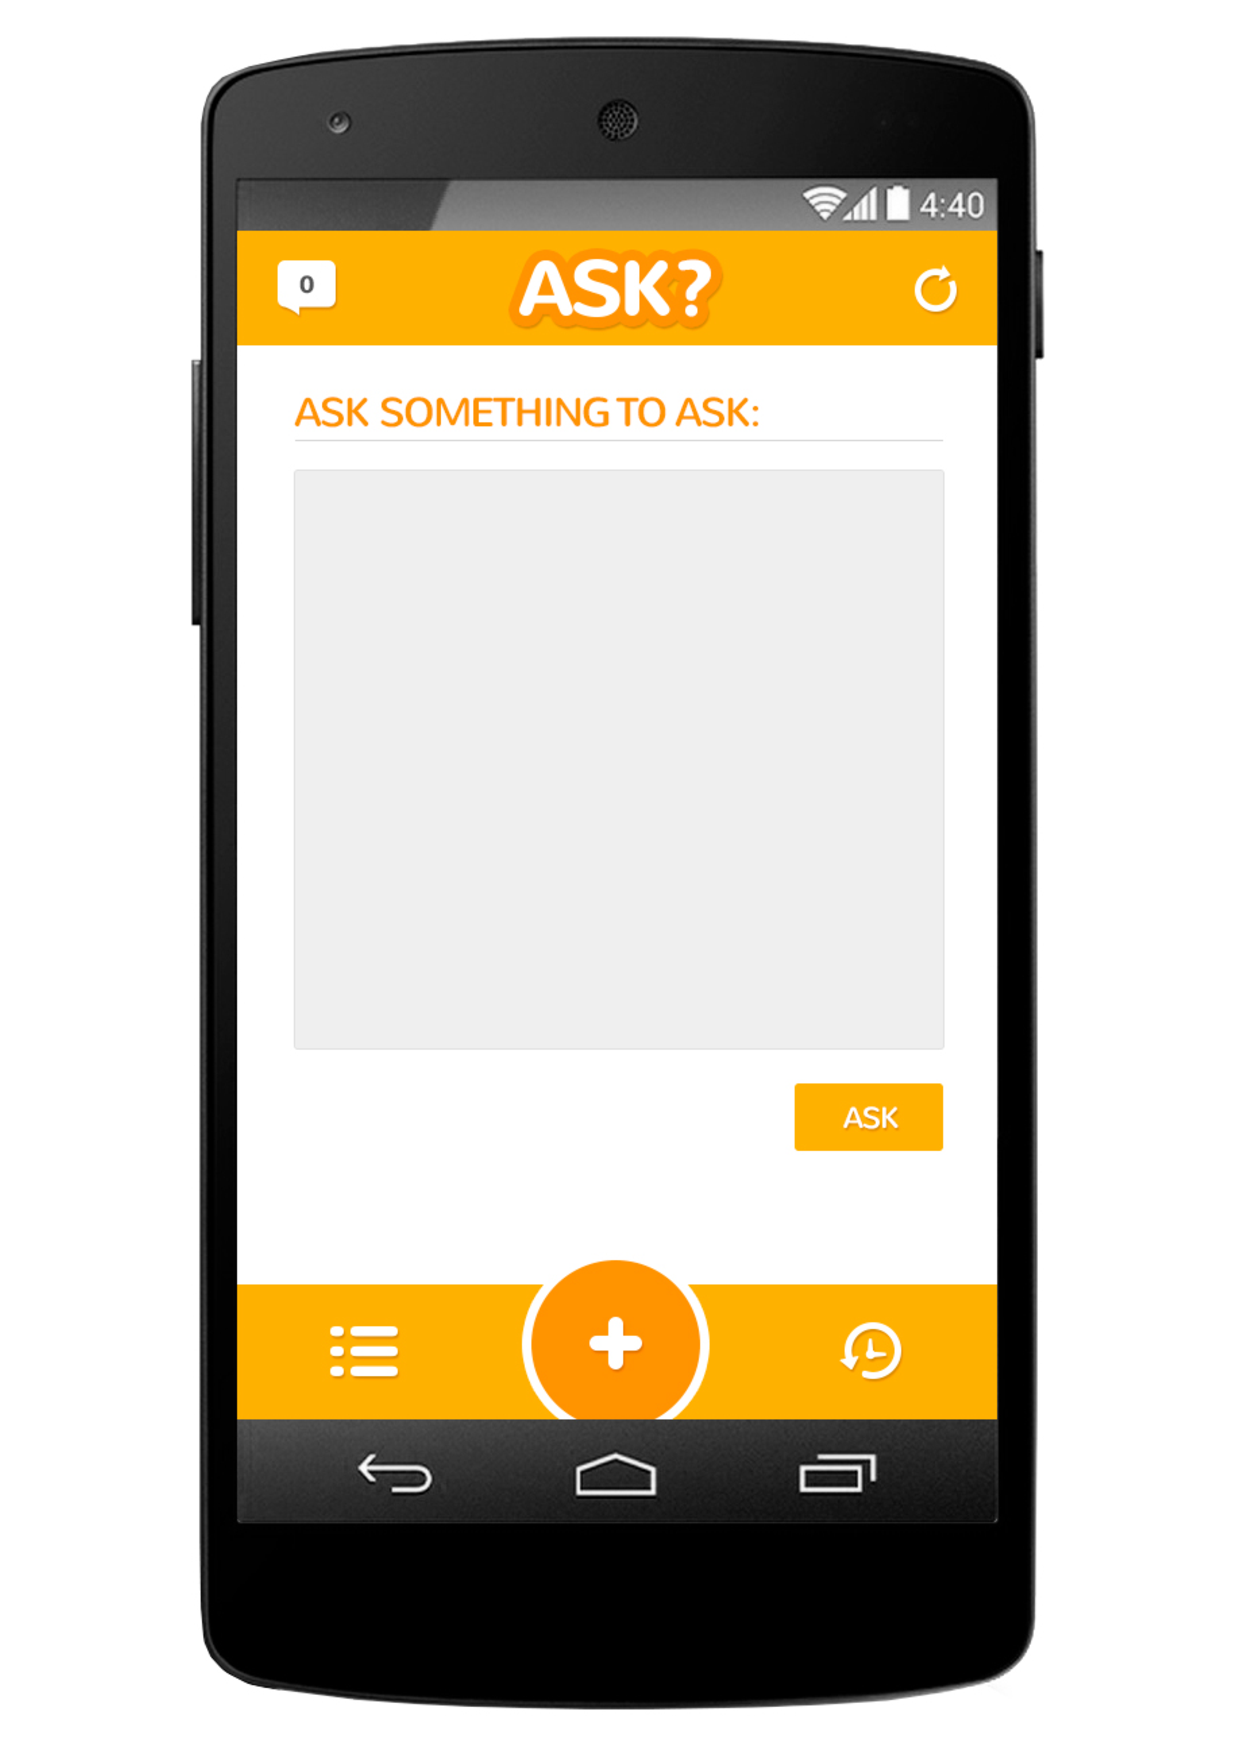
\includegraphics[width=0.2\textwidth]{./figs/ask/ask0.pdf}
    }
    \hfill
    \subfloat[Questions list\label{subfig-2:dummy}]{%
      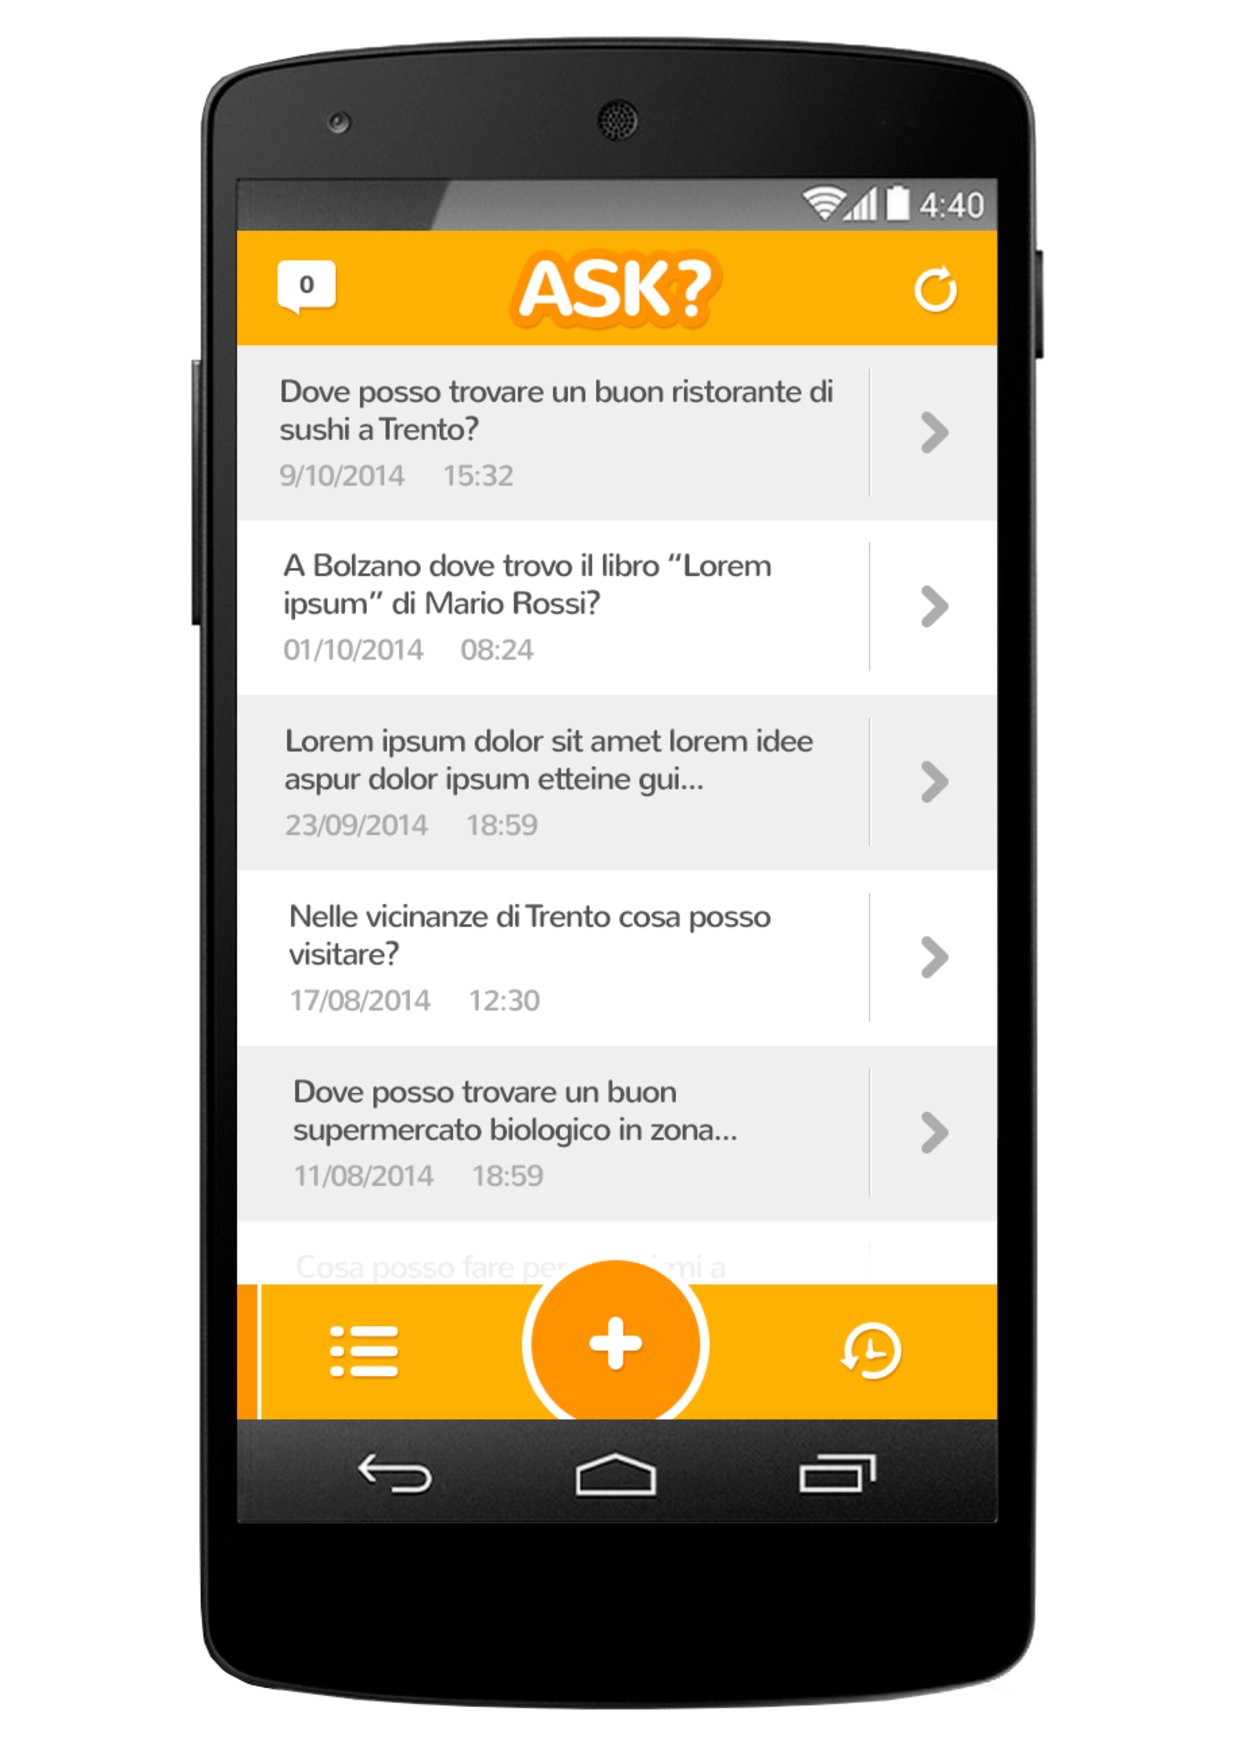
\includegraphics[width=0.2\textwidth]{./figs/ask/ask1.pdf}
    }
	\subfloat[Question\label{subfig-3:dummy}]{%
      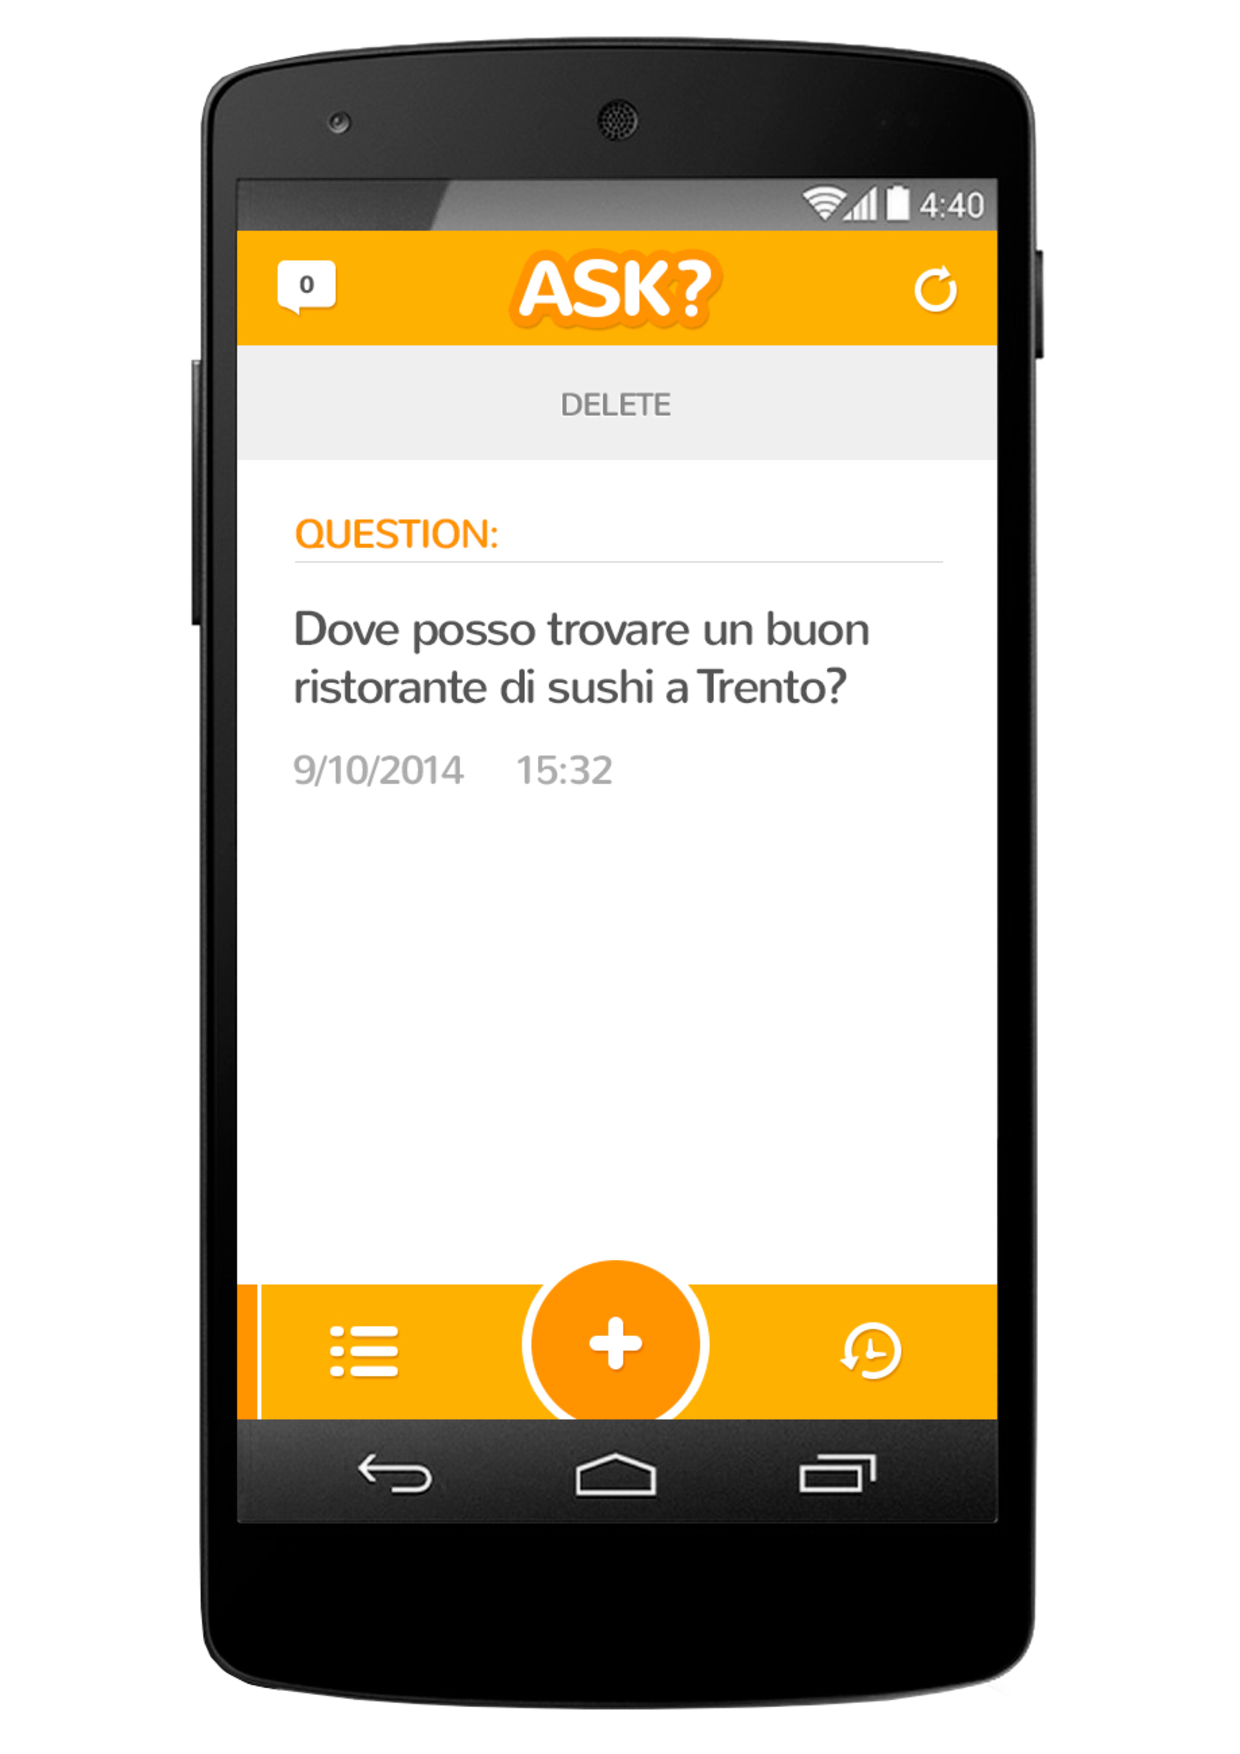
\includegraphics[width=0.2\textwidth]{./figs/ask/ask2.pdf}
    }
    	\subfloat[Question status\label{subfig-4:dummy}]{%
      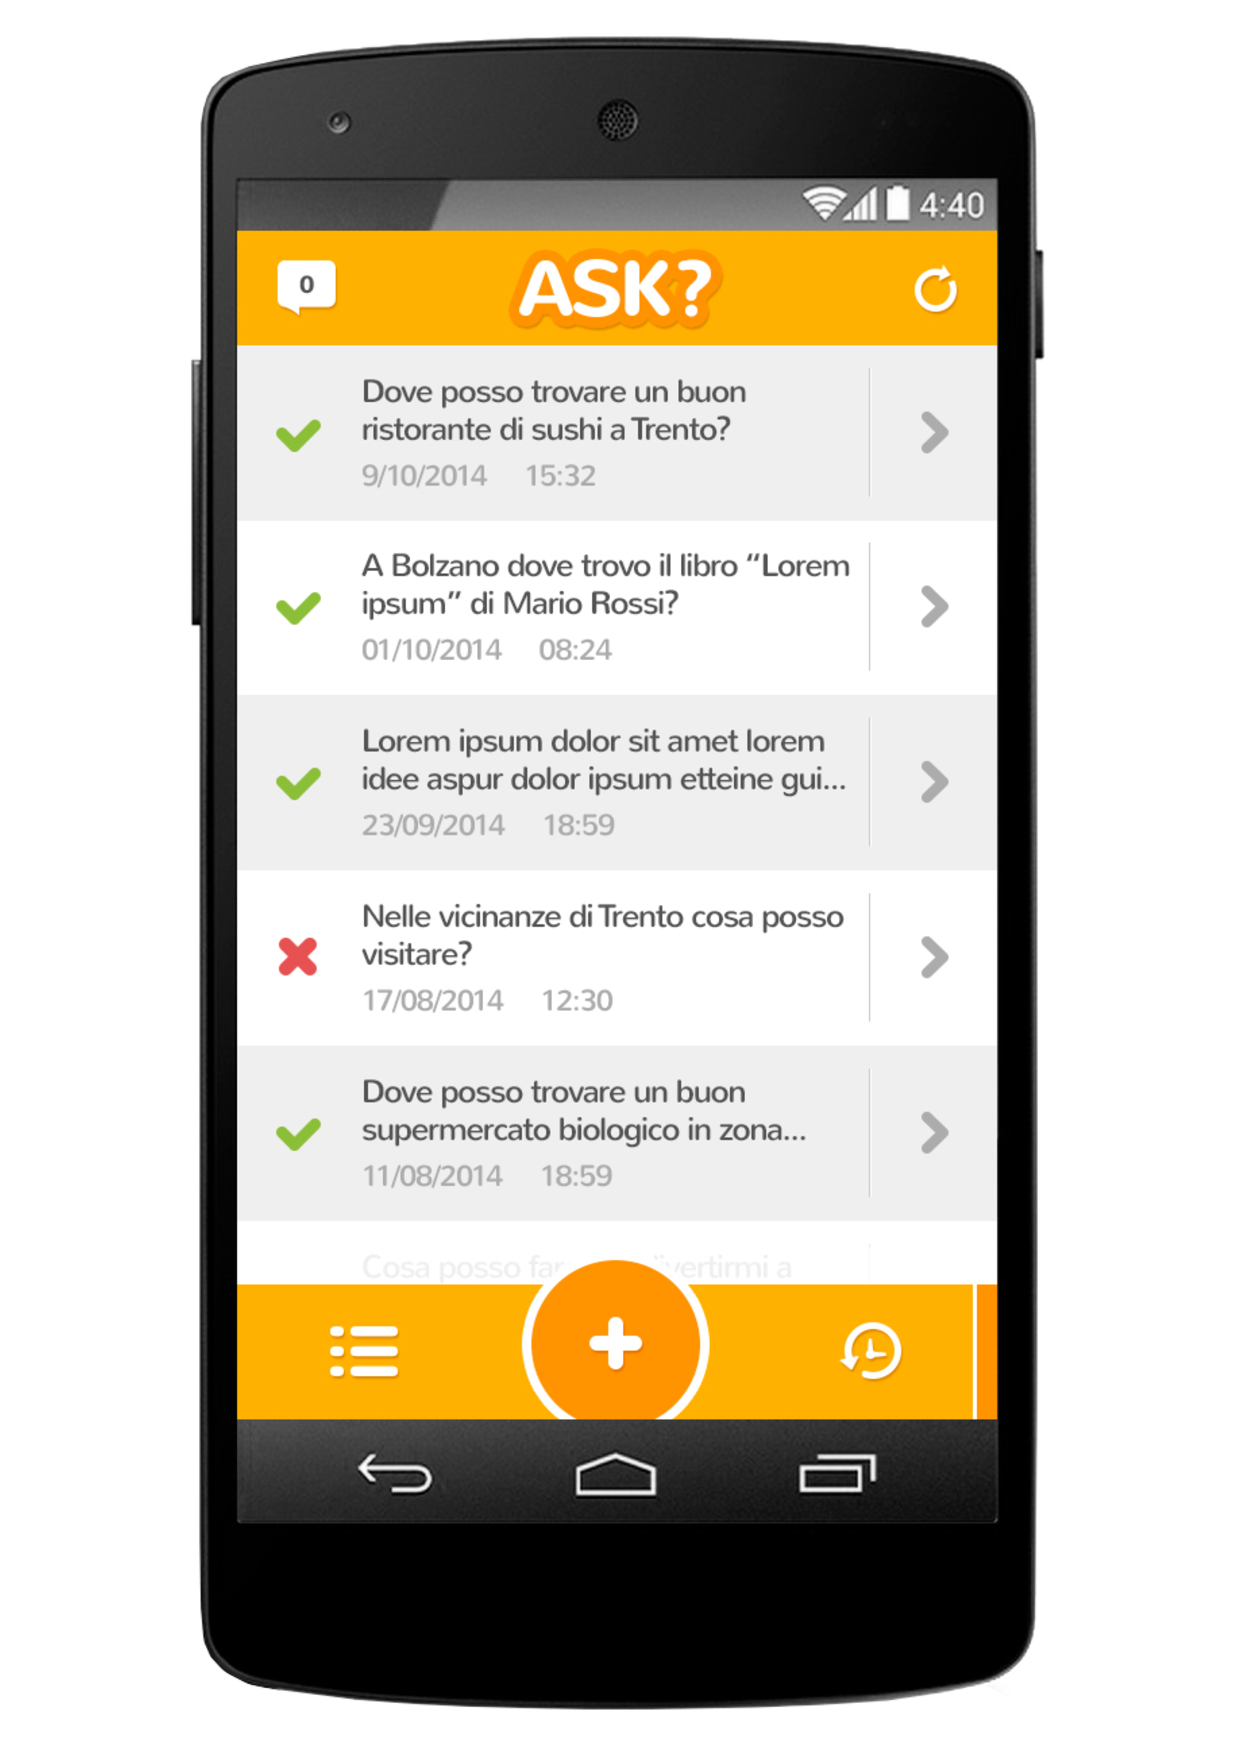
\includegraphics[width=0.2\textwidth]{./figs/ask/ask3.pdf}
    }
    	\subfloat[Answer details\label{subfig-5:dummy}]{%
      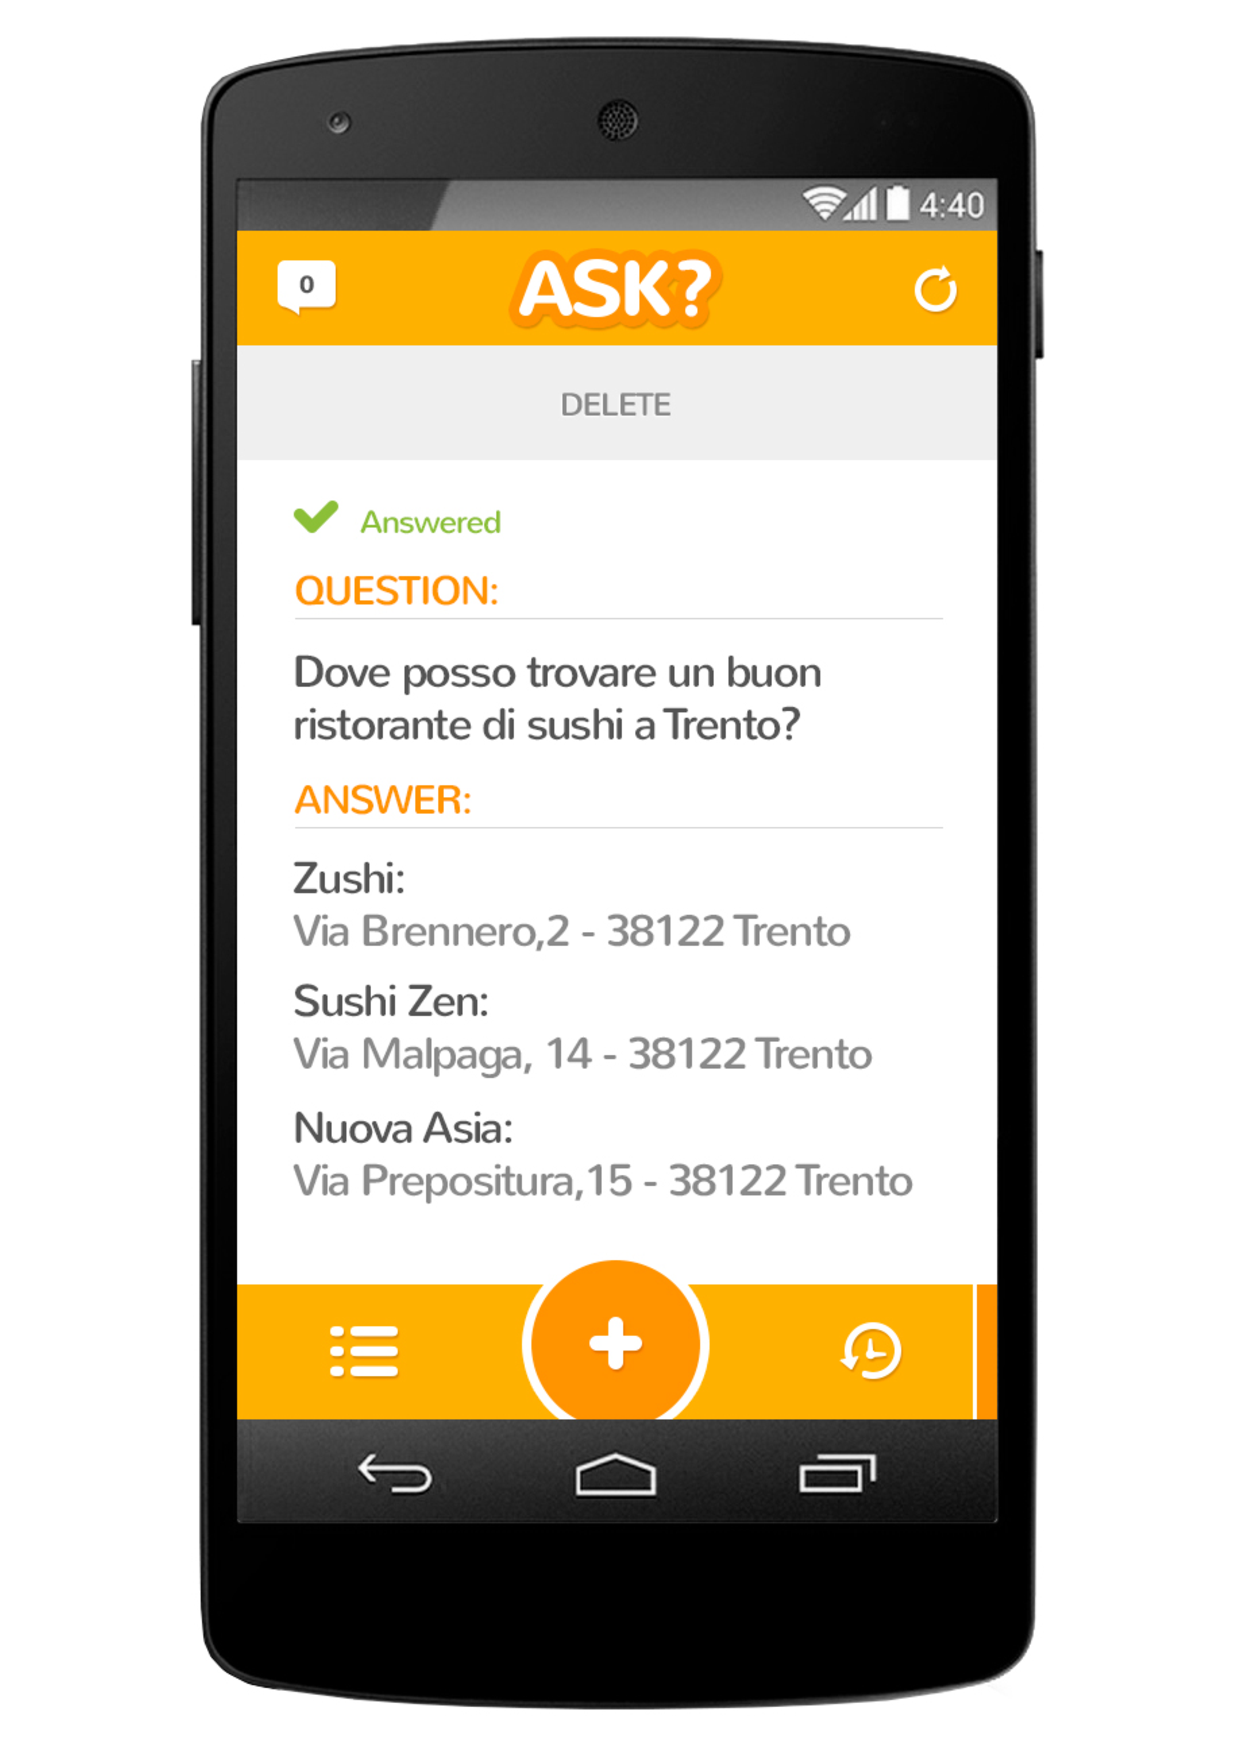
\includegraphics[width=0.2\textwidth]{./figs/ask/ask4.pdf}
    }
    \caption{Ask SmartSociety UX design}
    \label{fig:askpeer}
\end{figure}


\subsection{Example: SmartShare}
\textit{SmartShare} is a ridesharing application in which travellers share a vehicle for a trip and split travel costs such as gas, toll, and parking fees with others that have similar itineraries and time schedules. 
SmartShare reflects important features of HDA-CAS. First, it is a hybrid system, featuring humans who negotiate and perform physical rides as well as machines (intelligent software agents) that recommend routes, match people and monitor rides. SmartShare supports diversity awareness, in terms of users with different preference and affordances as well as different local cultures and values. SmarthShare supports collectives, in terms of both different types of using forming different communities as well as creating geographical clusters of activity. 
%They are diverse, supporting participants who are distributed geographically, come from different backgrounds and have different roles (e.g., driver, passenger). Participants have different travel requirements and preferences and access to different types of information. These aspects interact. For example, while large numbers of participants create more opportunities for participants, they also make it more difficult to allocate rides in an efficient, timely way.
 
%Given these qualities, SmartShare is a perfect setting within which to engage in SmartSociety research as it allows us to study key research questions addressed by the project.

The SmartShare sequence diagram is depicted in Fig.~\ref{fig:smartshare}. Users can post, by using the appropriate app interface, a ride request or ride offer. This includes information on the date, time and destination, as well a set of user preferences (e.g., 'I do not want a driver who smokes in the car') . This request is taken over by the orchestration manager. Constraints matching takes place within the OM, which creates a (plurality of) composition(s), in terms of peers matching constraints, and therefore constituting a potential ride. In the process of finding viable matches, the OM uses the search functionality exposed by the PM. 
%This information, together with the profile of the requesting user, are used by the SmartShare application to create a composition: peers matching both request constraints and user profile are identified and returned as a possible composition. 
The application then goes, using the OM functionality, through the recruitment (negotiation) process, in which each peer identified in the composition is contacted over the preferred communication channel and asked to confirm the participation in the ride. Peers provide individual ride agreement. If all intended peers provide a confirmation, the ride is fully agreed and execution can start. Execution can involve a number of steps, whose transitions are managed by the Execution Manager. Each step may include feedback from the users/peers. 
% Once the negotiation is successfully completed, an agreed ride plan is created, and the task execution (i.e., the actual ride) can take place. 
%This will happen asynchronously with respect to the initial request, on the date and time for which the ride share was searched. Once the ride share is executed the task is concluded.  

\begin{sidewaysfigure}
%\begin{figure}
\centering
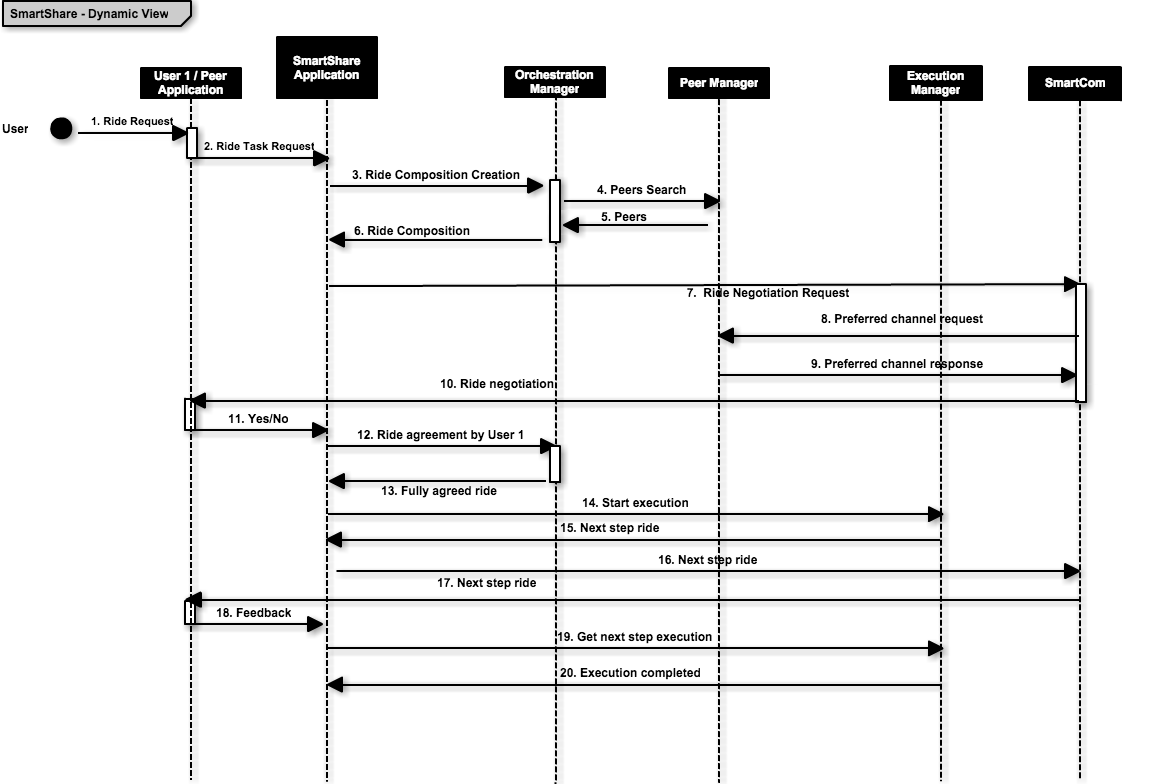
\includegraphics[width=0.9\textwidth]{./figs/sequenceRide}
\caption{Sequence diagram for SmartShare.}
\label{fig:smartshare}
\end{sidewaysfigure}

% %%%%%%%%%%%%%%%%%%%%%%%%%%%%%%%%%%%%%%%%%%%%%%%%%%%%%%%%%%%%%%
% \newpage

% %%%%%%%%%%%%%%%%%%%%%%%%%%%%%%%%%%%%%%%%%%%%%%%%%%%%%%%%%%%%%%
% \section{Interfaces Specifications}
% \label{sec:apis}
% In this section we will list the components integrated in the current
version of the SmartSociety platform and the key APIs thereof
used for supporting the two scenarios described in the previous
section.

\subsection{Peer Manager}
%The Peer Manager (PM) is developed within WP4 and its description can
%be found in Deliverable D4.2~\cite{D4.2} . 
The Peer Manager APIs specifications can be found at
\url{http://demos.disi.unitn.it:8080/smartsociety-score-api/} and are further
described in Deliverable D4.2~\cite{D4.2}. The PM is used for:
\begin{itemize}
\item {\bf Retrieving peers satisfying some requirements}: This
  request is made by the Orchestration Manager in order to identify
  potential peers composing a suitable collective for carrying out a
  given task. Endpoint used:\\
	\url{/instances/search/} (\textsc{GET})
\item {\bf Creating collective}: This request is made by the Application/Application Runtime at the end of the negotiation. Endpoint used:\\
	\url{/instances/} (\textsc{POST})
\item {\bf Retrieving peers in a collective}: This request is made by
  the Smartcom CM, so that it will be able to retrieve peer information later. Endpoint used:\\
	\url{/instances/search} (\textsc{GET})
\item {\bf Retrieving peers info}: This request is made by Smartcom, that requires the information about the communication channel to be used. Endpoint used:\\
	\url{/instances/search} (\textsc{GET})	
\end{itemize}


\subsection{Communication Middleware}
%The SmartCom Communication Middleware is developed within WP7 and its
%description can be found in Deliverable D7.1~\cite{D7.1}. 
The SmartCom Communication Middleware APIs specifications can be found at 
\url{https://github.com/tuwiendsg/SmartCom} and are further described in Deliverable D7.1~\cite{D7.1}. The Communication Middleware is mainly used for:
\begin{itemize}
\item {\bf Application to peer communication}: The Smart Society application sends messages to the peers belonging to a collective through Smartcom, that will deliver it using the preferred communication channel declared in the peer profile.
\item {\bf Peer to application reply communication}: Peers can reply to messages from the application. The platform provides an endpoint to which the peers can send a reply to a given message. The message is identified by the conversation id, this attribute is also used to know which application.
originally created the message, so that the platform can correctly dispatch it. 
\end{itemize}

\subsection{Orchestration Manager}
%The Orchestration Manager (OM) is developed within WP6 and its
%description can be found in  Deliverable D6.2~\cite{D6.2}. 
The Orchestration Manager APIs specifications can be found at
\url{https://bitbucket.org/rovatsos/smartsociety-internal/wiki/PeerManager/APIBGU}
and are further described in Deliverable D6.2~\cite{D6.2}. \\
In general, the various operations that the OM supports can be divided
into two big groups, depending on whether they require synchronisation
on the back-end or not:
\begin{itemize}
\item Operations that are read-only, and thus no synchronisation is
  needed on the documents on the backend;\
\item Operations that require write-operations, and thus
  synchronisation is critical and should happen on the backend
  (potentially by using semaphores and other approaches developed
  within WP6).
\end{itemize}
The key OM operations are:
\begin{itemize}
\item {\bf Posting a new task request}: In order to post a task request the following endpoint is used:\\
	\url{/applications/:app/taskRequests} (\textsc{POST})
\item {\bf Querying task requests:} The Smart Society application polls the orchestration manager to know the composition/negotiation state of the request. Endpoint used:\\
  \url{/applications/:app/taskRequests/:request_id} (\textsc{GET})
\item {\bf Querying tasks:} The Smart Society application retrieve the negotiable tasks to know which peer to contact for the negotiation. Endpoint used:\\
  \url{/applications/:app/tasks/:task_id} (\textsc{GET})
\item {\bf Updating tasks:} The Smart Society application updates the task according to whether the peer accepted or rejected it. Endpoint used:\\
  \url{/applications/:app/negotiations} (\textsc{PUT})
\end{itemize}

% %%%%%%%%%%%%%%%%%%%%%%%%%%%%%%%%%%%%%%%%%%%%%%%%%%%%%%%%%%%%%%
% \newpage


%%%%%%%%%%%%%%%%%%%%%%%%%%%%%%%%%%%%%%%%%%%%%%%%%%%%%%%%%%%%%%
\section{Prototype Description}
\label{sec:sw}
\todo{@Tommaso: rewrite the section, draw material from the CollaborateCom paper}
At the moment the platform mainly consists of a runtime allowing the Smart Society application to manage the submission of tasks by the user application. The platform provides also some library (against which the application is compiled) to operate with the current components (SmartCom, Orchestration Manager, Peer Manager). The code is in a private repository at \url{https://gitlab.com/smartsociety/appruntime}.%https://gitlab.com/Teudimundo/smartask}.

A Smart Society Application has its own identifier, generated during the registration phase. At the moment the application code is written by a developer directly in Java, in the final version the code will be generated through the programming framework. Each time a task is submitted to the application a new application instance is created, each instance has it's own state.

\subsection{Runtime}

When the runtime is run three endpoints are provided: 

\begin{itemize}
\item {\bf POST:/task/:applicationId/} To submit tasks, the runtime will ask the application to create a \textit{instance initializer} that will take care of the setup phase of the task. The application is expected to carry out all the operation that can be performed before interacting with the peers. The posted data is domain--dependent, and it will be serialized and managed by the application at the moment of instance creation. The runtime associated to the instance (hence the task) creates an identifier that is returned as response.

\item {\bf GET:/task/:applicationId/} To retrieve the status of all or part of the tasks of the application, query parameters can be used in the query and they will be managed by the application that might filter which tasks to show based non them. Note that the status format for each task is just required to be a valid json node (either a text or more complex structures), but it will be completely domain--dependent, in fact the SmartSociety application can send whatever information the user application requires.

\item {\bf GET:/task/:applicationId/:taskId} To retrieve the status of a specific task. As for the previous point both query parameters and the response are domain--dependent. 

\item {\bf POST:/message/:applicationId/} Used by the peer applications to communicate back with the application. To use this endpoint the application must have previously contacted the peer with a message containing a given conversation identifier. Such identifier is used then by the runtime to dispatch the message to the correct application instance, the content of the message is then handled by the application instance that  changes its state according to the information received.

\end{itemize}

\subsection{Component Library}

The component library allows the application development to be abstracted from the real components, allowing easier testing. 
Furthermore the component wrappers will give a simple interface to the component that is integrated with the runtime.


\subsection{Expected evolution}

In the future version of the platform each application and its runtime will be containerized. A service for routing the requests from general endpoints to the right application runtime will be provided.

The way the runtime will evolve, and its interaction with applications, is highly dependent on the outcome of the programming model and programming framework definition efforts currently ongoing within WP7.
%%%%%%%%%%%%%%%%%%%%%%%%%%%%%%%%%%%%%%%%%%%%%%%%%%%%%%%%%%%%%%
\newpage

\section{Prototype Validation and Testing}
\label{sec:val}
The final goal of validation activity is to test the ability of the platform to meet the high-level requirements %of the platform were 
described and analyzed in detail in~\cite{D8.1}. In Table~\ref{tab:req} we summarize the current status of the platform development in terms of ability to meet the requirements identified by the Consortium. As it can be seen, not all requirements have been met yet, in most cases as they refer to components which are still not fully completed within the respective workpackage. Yet, the platform in its current version already provides the minimum level of functionality required to handle a rather large range of social computations, as demonstrated by the available demo applications.

\begin{sidewaystable}
{\footnotesize \begin{tabular}{|p{1.2cm}|p{4cm}|p{6.5cm}|p{1.8cm}|p{5.4cm}|}
\hline \hline
ID & Chapter & Description & Met? & Remarks \\
\hline \hline
CR-1 & Computational Requirements & The platform should be able to execute human-based computations & Yes & See SmartShare and AskSmartSociety! demo\\  \hline
CR-2 & Computational Requirements & The platform should be able to execute machine-based computations & Yes & \\ \hline
CR-3 & Computational Requirements & The platform should be able to support hybrid computations & Yes & See AskSmartSociety! demo\\ \hline
PP-1 & Peer Profiles and Peer Profiling &: Peers will be characterized by a static and a dynamic profile. & Partially & See \cite{D4.1,D4.2,D4.3}, integration with context manager ongoing\\ \hline
PP-2 & Peer Profiles and Peer Profiling & Peer profiles data storage & Partially & See \cite{D4.3}  for integration with PPL\\ \hline
PP-3 & Peer Profiles and Peer Profiling & Peers can have multiple profiles & Partially & See \cite{D4.2,D4.3}\\ \hline
PP-4 &Peer Profiles and Peer Profiling  & Platform will support the profiling of peers & Partially & Integration with reputation service completed, full profiling missing\\ \hline
PU-1 & Platform Usability & The SmartSociety platform should be accessible through a set of open APIs & Partially & Final set of APIs will depend on the programming framework~\cite{D7.2} \\ \hline
PU-2 & Platform Usability & Ease for developers to create and manage applications & No & Depends on release of programming framework\\ \hline
PU-3 & Platform Usability & Support application development and deployment life-cycle automatically & Partially & A first version of the runtime is included in v2.0 \\ \hline
PU-4 & Platform Usability & Management GUI & Yes & The monitoring component has been integrated in v2.0 and includes a management dashboard\\ \hline
HT-1 & Platform Components and Interactions Heterogeneity & Number of different channels to interact with human peers & Yes & See~\cite{D7.1} and AskSmartSociety! demo.\\ \hline
HT-2 & Platform Components and Interactions Heterogeneity & Platform components will run on a variety of heterogeneous devices & No & Currently tested only on servers.\\ \hline
HT-3  & Platform Components and Interactions Heterogeneity & SmartSociety applications will be accessible via a variety of devices, online via the web and on mobile devices & Yes & See SmartSmare and AskSmartSociety! demos.\\ \hline
HT-4  & Platform Components and Interactions Heterogeneity & SmartSociety  will support a diversity of user interfaces for user engagement and recruitment & Partially & See~\cite{D9.3}\\ \hline
SEC-1 & Privacy and Security & Access Control & Partially & See~\cite{D4.3}\\  \hline
SEC-2 &  Privacy and Security & Trust and Reputation & Partially & Based on integration of the reputation service \\ \hline
SEC-3 &  Privacy and Security & Informed Consent & Partially & See~\cite{D4.3}\\ \hline
SEC-4 &  Privacy and Security & Peer Defined Usage Control Policies & No & \\ \hline
SEC-5 &  Privacy and Security & Secure Collection and Storage & Yes & See~\cite{D4.3}\\ \hline
SEC-6 &  Privacy and Security & Comprehensive explanations of security and privacy issues & No & \\ \hline
GOV-1 & Governance & Platform should support the collection of data related to governance & Partially & Provenance service integrated in v.2.0\\ \hline
GOV-2 & Governance  &Platform should support the implementation of governance policies & No & \\ \hline
PR-1 & Performance Requirements & Scalability & No & No scalability tests performed so far.\\ \hline
\end{tabular}
}
\caption{Features of platform 2.0 against requirements.}
\label{tab:req}
\end{sidewaystable}

We now move to briefly describing the validation and testing activities carried out within the scope of Task T8.4 ('Lab experiments and platform validation'). These were based on the flexible AskSmartSociety! application developed in year-2 and presented in~\cite{D8.2} and included the development of a number of small-scale prototypes aimed at testing the flexibility and extensibility of the platform. In particular, the following two results were achieved:
\begin{itemize}
\item {\bfseries Image tagging application:} based on the AskSmartSociety! application, a simple image tagging application was carried out. By means of such an application participants can post an image through the Ask! mobile application and ask other participants to provide tags representing the image content. Other participants can tag the image using the Reply! application or the SmartSociety twitter peer. Tags are collected in the AskSmartSociety! peer, where they are disambiguated (using a third-party semantic analysis engine), ranked and finally the most likely tags are reported back to the user. The development required minimal modifications of the Ask! and Reply! application, integration with a third-party service for entity extraction~\footnote{\url{https://dandelion.eu/}} and a third-party service for image storage~\footnote{\url{http://imgur.com/}}.
\item {\bfseries Facebook Peer and AskSmartSociety! Integration:} we developed a Facebook peer, in the form of a Facebook application connected to the SmartSociety platform. The integration was carried out for the AskSmartSociety! application. In this case, as it was for the Twitter peer, questions asked through the Ask! application get posted on the Facebook app page. Users who subscribed to the application can reply to the question using the 'comment' Facebook functionality. Additionally, users can 'like' comments posted by other users, an information which may be used to rank answers. In the AskSmartSociety! peer, answers from the Facebook peer are collected and integrated with those coming from the Reply! mobile app and the Twitter live feed. 
\end{itemize}
The work carried out to realize the two prototypes highlighted a number of issues in the current version of the platform, in particular in terms of functionality and ease of use of the APIs exposed by the Peer Manager; a new set of APIs was released by WP4 accordingly.
%%%%%%%%%%%%%%%%%%%%%%%%%%%%%%%%%%%%%%%%%%%%%%%%%%%%%%%%%%%%%%
\newpage


%%%%%%%%%%%%%%%%%%%%%%%%%%%%%%%%%%%%%%%%%%%%%%%%%%%%%%%%%%%%%%
\section{Discussion and Further Integration Steps}
\label{sec:concl}
The vision of the SmartSociety platform is to become an `IFTTT~\footnote{{\tt https://ifttt.com/}: IFTTT (IF This Then That) is a Web-based service allowing non-technical users to create chains of conditional statements (called `IF recipes') and actions (called `DO recipes') involving popular Web services.} for social computation', i.e., a platform that allows the easy integration of hybrid (human and machine) computational elements within the scope of a well-defined application workflow. While various steps have been taken in this direction, the overarching goal will require intense activities for the remainder of the project. 

Version 2.0 of the SmartSociety platform integrates seven key components: peer manager, orchestration manager, communication middleware, provenance service, reputation service, monitoring and analysis service and application runtime. This configuration is sufficient for developing a number of different applications using various types of social computation. Some limitations in terms of the single components are expected to be overcome with refinements from the relevant technical WP.

In terms of the upcoming steps, four major components to be integrated are the context manager (which will interact strictly with the peer manager), the reputation maanager, the task execution manager and the incentive server. Major changes in the platform configuration will come from the delivery of the programming framework by WP7 (foreseen at M36), which will have a major impact on how platform functionality can be accessed by application developers. Interactions with the virtual gamified environment in WP9 may also lead to a refactoring of some of the features exposed by the platform. Another major release of the platform is foreseen at M36. 

%In line with the DoW, the actual internal release of the first version of the platform (including user modules) represents MS18 and is due at M27. By M27 the integration roadmap foresees the integration of the provenance store and of the reputation manager. It will further include a fi5rst version of the execution manager and of the monitoring and analysis service. Security and privacy aspects will be integrated during the third year of the project, in particular within the scope of WP4 (where all personal information is stored). The programming framework development will be strictly aligned with the platform functionality enhancement and will support the easy registration and deployment of applications. The context manager will be integrated with the peer manager in the course of 2015. The incentives manager will be integrated in a later stage of the project, the actual integration date depending on the progress of research activities within WP5. Further work will be carried out in a dialogue with WP1 in terms of devising mechanisms supporting various governance models for the platform. Last, but not least, the development of the platform will also reflect the work on exploitation plans and potential business models carried out within the scope of WP10.

%The second platform prototype (including validation results from lab experiments) will be delivered as D8.3 at M30. 

% In this deliverable we have introduced:
% \begin{itemize}
% \item An analysis of requirements for the SmartSociety platform, elicited by working in  cooperation with the other work packages and covering both functional and non-functional properties. 
% \item A system-level architecture, encompassing:
% \begin{itemize}
% \item the definition of the logical and functional role of each platform component;
% \item a definition of the interactions among components;
% \item the preliminary identification of modules within each component, in line with the progress of single technical WPs.
% \end{itemize}
% \end{itemize}

% This document represents the starting point for the integration activities taking place in the second year of the project (T8.2 and T8.3). The overall architecture will be iteratively revised, improved and extended during the second year of the project, leading to the delivery, at M24, of a first prototypical implementation of the platform. D8.1 will
% serve as reference document and handbook for the development and prototyping activities to be carried out within WP2-WP7, defining clearly the role of the respective components in the overall platform architecture and the interaction patterns with other components. The architecture will be maintained as a living reference document; the release of the first prototype at M24 will go hand in hand with the provisioning of a revised architectural specification, accounting for the evolution of perspectives during year-2.

% Last, it is worth remarking that WP8 played an important {\it integration}
% role in the first year of activities of the SmartSociety project. In order to reach
% a consistent view on the architecture of the SmartSociety platform, indeed,
% WP8 established and fostered an active and open discussion among the
% technical WPs (WP2-WP7). The agreement reached among WPs in terms of logical role, functionalities of their components, and interaction patterns represents an important contribution of WP8 in year-1. 



%%%%%%%%%%%%%%%%%%%%%%%%%%%%%%%%%%%%%%%%%%%%%%%%%%%%%%%%%%%%%%
\newpage

%%%%%%%%%%%%%%%%%%%%%%%%%%%%%%%%%%%%%%%%
%%%%%%%%%%%%%%%%%%%%%%%%%%%%%%%%%%%%%%%%%%%%%%%%%%%%%%%%%%%%%%%%%%%%%%%%%%%%%%%%%%%%%%%%%%%%%%%%%%%%%%%%%%%%%%%%%%%%%%%%
\bibliographystyle{./IEEEtran}
\bibliography{BIB/biblio.bib}
%\clearpage
\appendix
\section{Monitoring component}\label{app:monitoring}
In the period M25-M30, the monitoring component was developed and integrated within the scope of WP8.\\
The monitoring framework is responsible for the monitoring of the overall SmartSociety platform and components. It acts as a central collection point for any information which is considered important to ensure the proper functioning of the platform. Target users of the monitoring components are system administrators who need to check the status of the system and the liveness of the services. 

The monitoring framework allows to:
\begin{itemize}
\item Dynamically collect diverse information relevant for monitoring the proper functioning of the platform and its performance. Such information is permanently stored in a non-relational database and available at any time for inspecting specific platform behaviors.
\item Visualize such information in real-time by means of interactive dashboards, or query the collected data via dedicated APIs. %In particular, through the Monitoring framework it is possible to create and configure specific visualizations starting from the data that has been collected. There can be multiple visualizations, each one geared towards a specific platform KPI or informative visualization.
\end{itemize} 

%first, it allows to permanently store the data that is collected from the various COMPOSE components. The information can then be explored over time in order to either analyse the performance of platform components, or identify the causes of a specific malfunctioning. 
%Second, it allows to visualize both real-time, as well historical data. In particular, through the Monitoring dashboard it is possible to create and configure specific visualizations starting from the data that is collected. There can be multiple visualizations, each one geared towards a specific platform KPI or information.
%The COMPOSE platform administrator is expected to be the key utilizer of the Monitoring Dashboard. The current implementation does not support different visualizations based on user role.

The high-level architecture of the monitoring component is represented in~\ref{fig:monitoringArch}.
%Monitoring Dashboard is based on the following architecture and components:


\begin{figure}[!hbt]
\centering
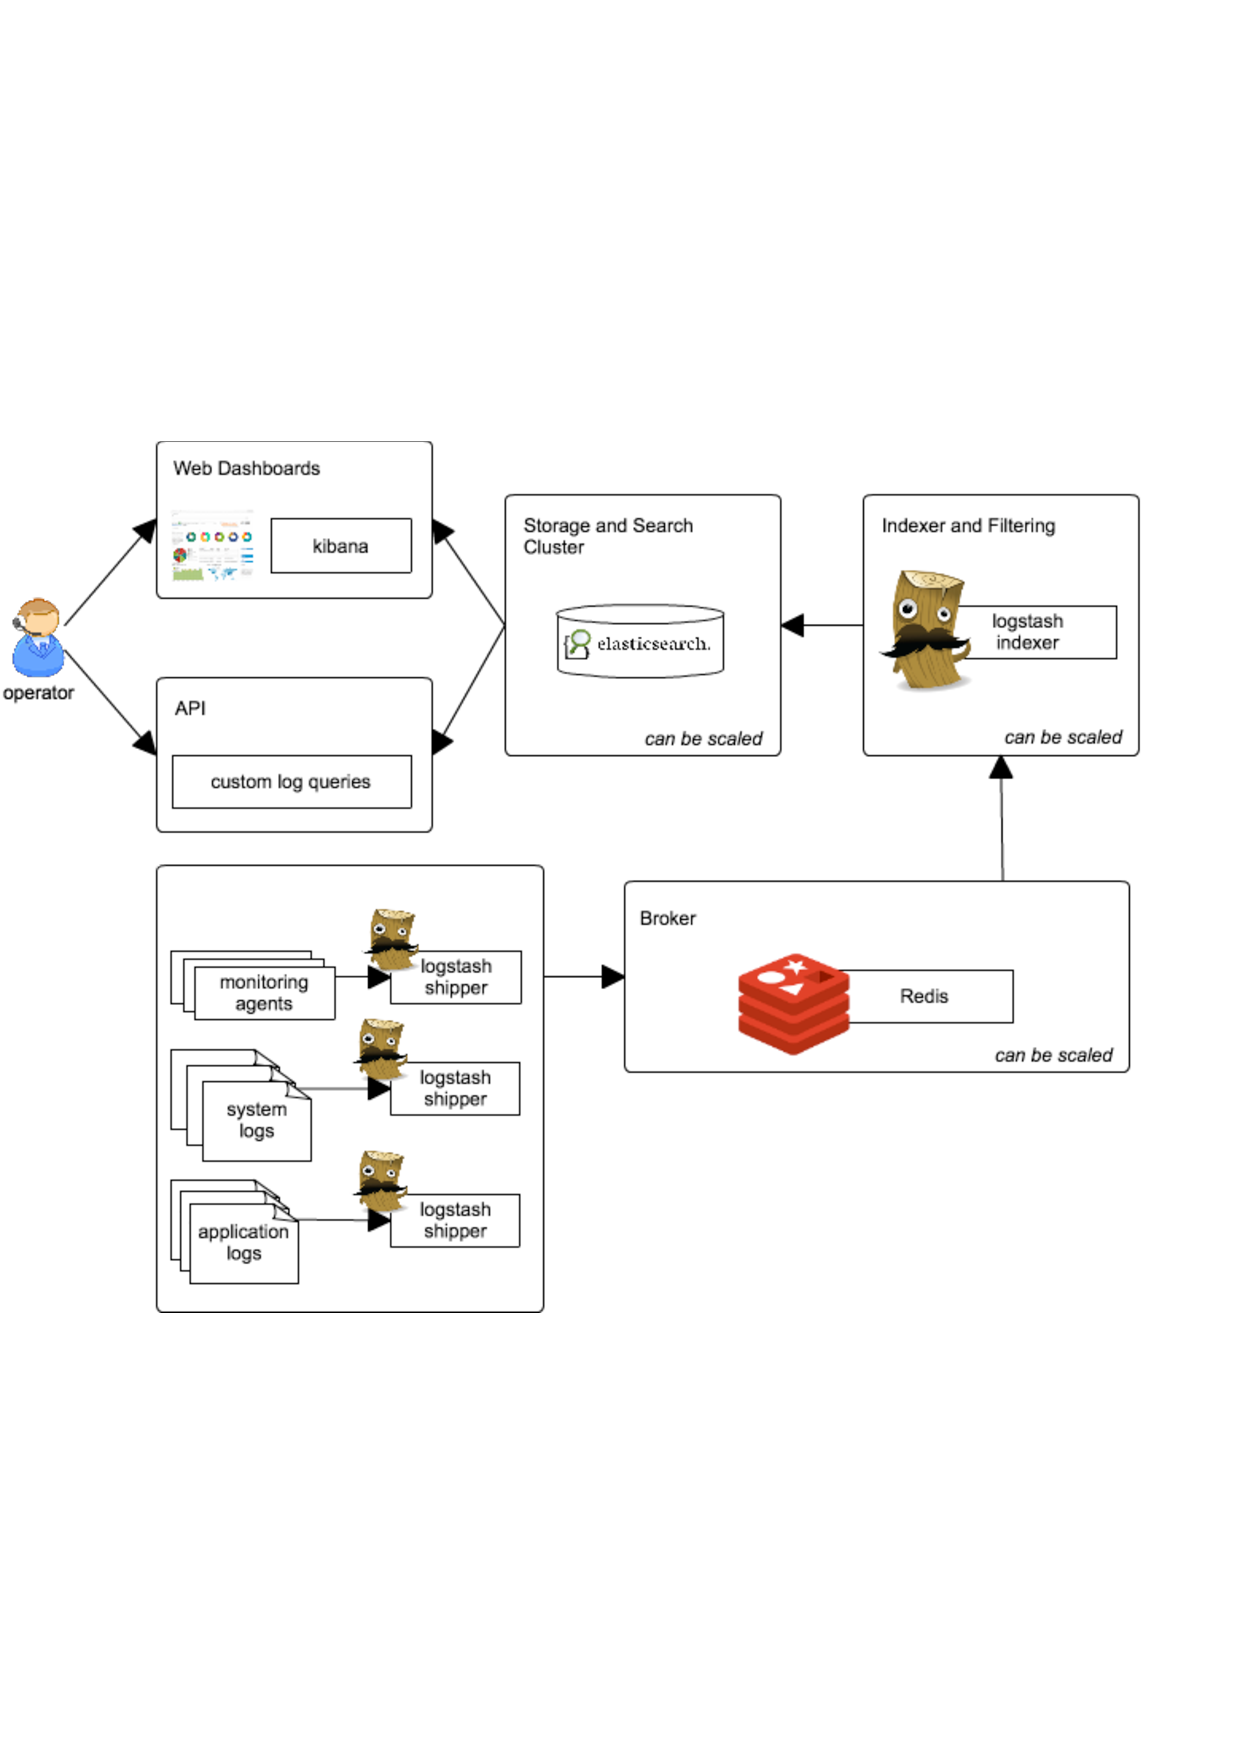
\includegraphics[width=0.8\textwidth]{figs/monitoring.pdf}
\caption{Monitoring framework architecture.}
\label{fig:monitoringArch}
\end{figure}

The monitoring framework is based on Logstash\footnote{{\tt http://logstash.net/}}, an open-source tool for managing events and logs. Logstash can be used to collect logs, parse them, and store them for later use (e.g., search and visualization). %Speaking of searching, Logstash comes with a web interface for searching and drilling into all of the logs collected over time.
It is possible to define what information shall be permanently stored and processed by the monitoring framework. In particular, it is possible to integrate:
\begin{itemize}
\item System logs: these logs correspond to logs, which are generated by the various system components such as, e.g., web servers, application servers. 
\item Application logs: specific logs that are produced by applications, and require a constant integration for debugging and monitoring purposes.
\item Monitoring information: any agent that can be configured to deliver data to the Logstash infrastructure.
\end{itemize}

In all three cases, a Logstash shipper is used to connect the specific source of data to Logstash. Specific shippers already exists for some widely used system components such as, e.g., web servers, databases, etc., while custom shippers can be created for specific cases. In the case of SmartSociety, we created a dedicated shipper to collect the events produced by the various platform components.\\
The following component is a Redis Broker. This is an optional component that can be used in order to scale the system to large volumes of events and data. Based on Redis, data is indexed in order to prepare it for optimal searching and querying. Once the data is indexed, it is stored in an ElasticSearch cluster for storage and search. 
Starting from the data stored in ElasticSearch, it is possible to build queries on scale to explore the collected data. We decided to use Kibana\footnote{{\tt https://www.elastic.co/products/kibana}} as the tool to create and visualize queries on the collected data. Kibana is fully integrated with ElasticSearch, and allows to easily explore and analyze large volumes of data. A sample visualization is shown in~\ref{fig:kibana}.  The metrics and specific charts can be configured dynamically by the administrator of the platform.

In addition, ElasticSearch provides APIs for querying and extracting the data stored in the platform. This can be helpful in the case aggregated views such as, e.g., monthly reports, are needed.

\begin{figure}[!hbt]
\centering
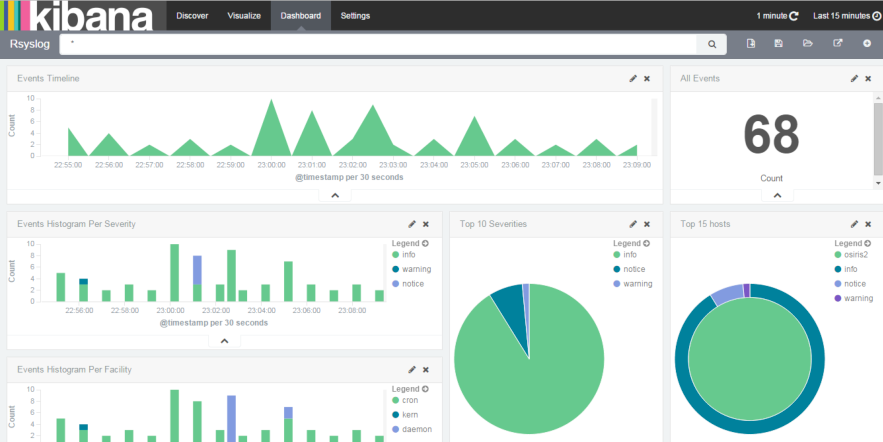
\includegraphics[width=0.8\textwidth]{figs/kibana.pdf}
\caption{Example of the monitoring framework web interface.}
\label{fig:kibana}
\end{figure}

\end{document}
